% TesisVG_Cap5.tex
% Capítulo 5: Método de Schröder en el plano complejo
\chapter{Método de Schröder en el plano complejo}
\label{cap:schroder_plano_complejo}

En este capítulo presentamos un estudio completo de la dinámica del método de Schröder en el plano complejo. Comenzamos introduciendo el método y sus propiedades fundamentales, para después analizar su comportamiento aplicado a polinomios con dos raíces de multiplicidades arbitrarias y, finalmente, extender el estudio a polinomios cúbicos mediante el análisis del plano de parámetros. Los resultados teóricos se ilustran mediante diagramas de cuencas de atracción que revelan la estructura fractal subyacente.

\section{Introducción: Método de Schröder y conceptos fundamentales}

\subsection{Definición del método de Schröder}

El método de Schröder fue introducido por Ernst Schröder en su trabajo seminal de 1870 \cite{Sch} sobre la resolución de ecuaciones no lineales. Schröder construyó este método aplicando el método de Newton a la ecuación $\tfrac{f(z)}{f'(z)}=0$, obteniendo el esquema iterativo
\begin{equation}
 z_{k+1}=S_f(z_k)=z_k-\frac{f(z_k)f'(z_k)}{f'(z_k)^2-f(z_k)f''(z_k)}, \quad k\ge 0, \quad z_0\in\C.
 \label{eq:Sch_def}
\end{equation}
Una ventaja importante del método de Schröder, señalada por el propio autor, es que converge cuadráticamente incluso para raíces múltiples, a diferencia del método de Newton que reduce su orden de convergencia en presencia de multiplicidad.

Para mayor comodidad, podemos escribir el iterador de Schröder en términos de la función
\begin{equation}
 L_f(z)=\frac{f(z)f''(z)}{\big(f'(z)\big)^2}
 \label{eq:Lf_def}
\end{equation}
como
\begin{equation}
 S_f(z)=z-\frac{1}{1-L_f(z)}\,\frac{f(z)}{f'(z)}.
 \label{eq:Sch_real}
\end{equation}

El coste computacional del método de Schröder es superior al de Newton: requiere evaluar no solo $f$ y $f'$, sino también $f''$, lo que lo sitúa en un nivel de coste comparable a los métodos de la familia Chebyshev-Halley.

% \subsection{Conjugación topológica}

% Una herramienta fundamental en el análisis de sistemas dinámicos es la conjugación topológica. Dos funciones $f,g: \C \to \C$ se dicen \emph{topológicamente conjugadas} si existe un homeomorfismo $\varphi$ tal que
% $$
% \varphi\circ g=f\circ \varphi.
% $$
% La conjugación topológica es muy útil porque funciones conjugadas comparten las mismas propiedades dinámicas desde el punto de vista topológico: los puntos fijos de una función se mapean en puntos fijos de la otra, los puntos periódicos corresponden entre sí, y lo mismo ocurre con las cuencas de atracción y los conjuntos de Julia.

% \subsection{El problema de Cayley para polinomios cuadráticos}

% En 1879, Arthur Cayley \cite{Cay} abordó el problema de caracterizar las cuencas de atracción del método de Newton aplicado a polinomios cuadráticos con raíces simples. Este problema, conocido como el \emph{problema de Cayley}, estableció las bases para el estudio de la dinámica compleja de métodos iterativos.

% Cayley demostró que para el polinomio
% \begin{equation}
% f(z)=(z-a)(z-b),\quad a,b\in \C, \quad a\ne b,
% \label{eq:poly_simple}
% \end{equation}
% la función iterativa de Newton es conjugada con la función $R(z)=z^2$ mediante una transformación de Möbius. El conjunto de Julia es la bisectriz entre las raíces $a$ y $b$, y las cuencas de atracción son los dos semiplanos correspondientes.

% De manera análoga, el método de Schröder aplicado al mismo polinomio es conjugado con $-R(z)=-z^2$, produciendo el mismo conjunto de Julia y las mismas cuencas de atracción. Esto muestra que, para polinomios cuadráticos con raíces simples, ambos métodos tienen comportamiento dinámico idéntico.

\section{Polinomios con dos raíces de multiplicidades arbitrarias}

Consideramos ahora el caso más general de polinomios con dos raíces complejas de multiplicidades distintas:
\begin{equation}
 f(z)=(z-a)^m(z-b)^n,\qquad a,b\in\C,\ a\ne b,\quad m\ge n\ge 1.
 \label{eq:poly_dos_raices}
\end{equation}
Este caso es significativamente más interesante que el de raíces simples, pues la presencia de multiplicidades distintas rompe la simetría y produce conjuntos de Julia con geometría circular no trivial.

\subsection{Reducción al caso canónico mediante conjugación}

Para simplificar el análisis, realizamos una conjugación afín que traslada las raíces $a$ y $b$ a $1$ y $-1$ respectivamente. Definimos la transformación afín
\begin{equation}
A(z)=1+2\frac{z-a}{a-b}
\label{eq:afin}
\end{equation}
y consideramos la función conjugada
\begin{equation}
T_{m,n}(z)=A\circ S_f\circ A^{-1}(z)=\frac{(m-n) z^2 +2 (m+n) z +m-n}{(m+n) z^2 +2(m-n)z +m+n}.
\label{eq:Tmn}
\end{equation}
Esta función $T_{m,n}$ representa la dinámica del método de Schröder aplicado a $(z-1)^m(z+1)^n$ y depende únicamente de las multiplicidades $m$ y $n$.

Mediante una segunda conjugación con la transformación de Möbius
\begin{equation}
M(z)=\frac{z-1}{z+1}
\label{eq:Mobius}
\end{equation}
llegamos a una función racional extremadamente simple:
\begin{equation}
R_{m,n}(z)=M\circ T_{m,n}\circ M^{-1}(z)=-\frac{n}{m}z^2.
\label{eq:Rmn}
\end{equation}

\subsection{Análisis dinámico de $R_{m,n}$}

La función $R_{m,n}(z)=-\tfrac{n}{m}z^2$ tiene una dinámica completamente caracterizada. El círculo
$$
C_{m,n}=\left\{z\in\C; |z|=\frac{m}{n}\right\}
$$
es invariante bajo $R_{m,n}$. Los puntos con $|z_0|<m/n$ convergen al origen bajo iteración, mientras que los puntos con $|z_0|>m/n$ divergen a infinito. Por tanto, $C_{m,n}$ es el conjunto de Julia de $R_{m,n}$.

\subsection{Teoremas principales: caracterización del conjunto de Julia}

Los siguientes dos teoremas constituyen los resultados principales de este capítulo, caracterizando completamente el conjunto de Julia del método de Schröder para polinomios con dos raíces.

\begin{teorema}[Conjunto de Julia en el caso canónico]
\label{teo:julia_canonico}
Sea $T_{m,n}(z)$ la función racional definida por \eqref{eq:Tmn} y sea $J_{m,n}$ su conjunto de Julia. Entonces:
\begin{enumerate}
\item Si $m=n$, entonces $J_{m,m}$ es el eje imaginario.
\item Si $m>n\ge 1$, entonces $J_{m,n}$ es el círculo
\begin{equation}
J_{m,n}=\left\{z\in\C; \left|z+\frac{m^2+n^2}{m^2-n^2}\right|=\frac{2mn}{m^2-n^2}\right\}.
\label{eq:Julia_canonico}
\end{equation}
\end{enumerate}
\end{teorema}

\begin{proof}
La demostración se sigue inmediatamente del análisis de la dinámica de $R_{m,n}$. El conjunto de Julia $J_{m,n}$ es la preimagen del círculo $C_{m,n}=\{z\in\C; |z|=m/n\}$ bajo la transformación de Möbius $M(z)=(z-1)/(z+1)$.

Para el caso $m=n$, tenemos $C_{m,m}=\{z\in\C; |z|=1\}$ y su preimagen por $M$ es el eje imaginario.

Para $m>n$, la preimagen del círculo $|z|=m/n$ por $M$ es un círculo en el plano $z$ cuyo centro y radio se calculan mediante transformación conforme. Distinguiendo los casos según las distintas configuraciones del círculo de partida, se obtiene la expresión explícita \eqref{eq:Julia_canonico}.
\end{proof}

\begin{teorema}[Conjunto de Julia para raíces arbitrarias]
\label{teo:julia_general}
Sea $S_f(z)$ la función iterativa del método de Schröder aplicado a polinomios \eqref{eq:poly_dos_raices} y sea $J_{m,n,a,b}$ su conjunto de Julia. Entonces:
\begin{enumerate}
\item Si $m=n$, entonces $J_{m,m,a,b}$ es la recta equidistante entre los puntos $a$ y $b$.
\item Si $m>n\ge 1$, entonces $J_{m,n,a,b}$ es el círculo
\begin{equation}
J_{m,n,a,b}=\left\{z\in\C; \left|z+\frac{b m^2-a n^2}{m^2-n^2}\right|=\frac{mn |a-b|}{m^2-n^2}\right\}.
\label{eq:Julia_general}
\end{equation}
\end{enumerate}
\end{teorema}

\begin{proof}
Este resultado se deduce calculando la preimagen de $J_{m,n}$ bajo la transformación afín $A(z)$ definida en \eqref{eq:afin}. La transformación afín preserva círculos y rectas, y traslada y escala el conjunto de Julia canónico al caso general con raíces $a$ y $b$. Los parámetros del círculo se obtienen aplicando la transformación afín a los parámetros del caso canónico.
\end{proof}

\subsection{Cuencas de atracción}

La caracterización del conjunto de Julia permite determinar completamente las cuencas de atracción:

\begin{itemize}
\item En el caso $m=n$, la cuenca de atracción de cada raíz es un semiplano delimitado por la recta equidistante entre ambas raíces.

\item En el caso $m>n$, el interior del círculo $J_{m,n,a,b}$ constituye la cuenca de atracción de la raíz de menor multiplicidad $b$, mientras que el exterior (incluyendo el infinito) es la cuenca de atracción de la raíz de mayor multiplicidad $a$.
\end{itemize}

Este resultado muestra un fenómeno interesante: la cuenca de atracción de la raíz de mayor multiplicidad ``rodea'' a la cuenca de la raíz de menor multiplicidad, que queda confinada en un disco.

\subsection{Análisis paramétrico: influencia de la razón de multiplicidades}

Introduciendo el parámetro $p=m/n$, que representa la razón entre las multiplicidades, podemos expresar los círculos $J_{m,n}$ como
\begin{equation}
J_{p}=\left\{z\in\mathbb{C}; \left|z+\frac{p^2+1}{p^2-1}\right|=\frac{2p}{p^2-1}\right\}.
\label{eq:Julia_param}
\end{equation}

Esta expresión muestra que todos los polinomios $(z-1)^m(z+1)^n$ con el mismo cociente $p=m/n$ tienen el mismo conjunto de Julia para el método de Schröder. Esto simplifica considerablemente el análisis paramétrico.

\subsection{Comportamiento asintótico}

Podemos esquematizar la dinámica del método de Schröder aplicado a polinomios $(z-1)^m(z+1)^n$, $m>n$ de la siguiente manera:

\begin{itemize}
\item \textbf{Cuando $p=m/n\to \infty$:} Los centros de los círculos $J_p$ tienden a $-1$ (la raíz de menor multiplicidad) y los radios tienden a cero. Es decir, el conjunto de Julia se colapsa en un punto coincidente con la raíz simple. La cuenca de atracción de la raíz múltiple domina casi todo el plano complejo.

\item \textbf{Cuando $p=m/n\to 1^+$:} Los centros
$$
-\frac{p^2+1}{p^2-1}\to -\infty \text{ cuando } p\to 1^+
$$
y los radios
$$
\frac{2p}{p^2-1}\to \infty \text{ cuando } p\to 1^+.
$$
Por tanto, los círculos crecen indefinidamente y tienden a ``explotar'' en el caso límite $p=1$, recuperando el eje imaginario que corresponde al caso de multiplicidades iguales.
\end{itemize}

Si consideramos la presencia de raíces arbitrarias $a$ y $b$, la dinámica del método de Schröder aplicado a polinomios $(z-a)^m(z-b)^n$, $m>n$ puede resumirse como un ``viaje'': partiendo de un círculo concentrado en la raíz de menor multiplicidad $b$ (cuando $p\to\infty$), pasando por círculos con centro en la línea que conecta las raíces $a$ y $b$ y radio creciente, hasta la ``explosión'' en la bisectriz de ambas raíces cuando $p=1$.

\subsection{Ilustraciones: cuencas de atracción}

A continuación presentamos diagramas de cuencas de atracción que ilustran los resultados teóricos obtenidos. En todas las figuras se compara el comportamiento del método de Schröder con el del método de Newton aplicados a los mismos polinomios. Las regiones de color corresponden a las cuencas de atracción de cada raíz.

\subsubsection{Caso: $p=m/n$ creciente}

En la Figura~\ref{fig:p_creciente} se muestra el comportamiento cuando la razón $p=m/n$ aumenta. Se aplican ambos métodos a polinomios $(z-1)^m(z+1)^n$ con $n=1$ fijo y $m$ creciente.

\begin{figure}[H]
\centering 
\begin{minipage}[t]{0.45\textwidth}
\centering
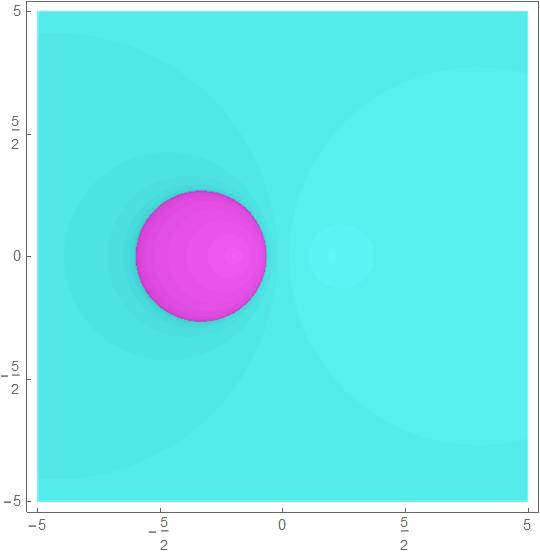
\includegraphics[width=0.98\textwidth]{fuentes/articulo-cuadraticos/imagenes/sch_m_2n_1.jpg}
\small Schröder: $m=2, \, n=1.$
\end{minipage}\hfill
\begin{minipage}[t]{0.45\textwidth}
\centering
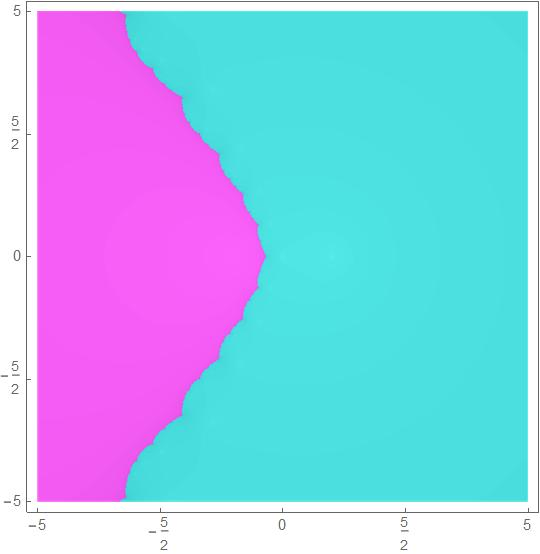
\includegraphics[width=0.98\textwidth]{fuentes/articulo-cuadraticos/imagenes/newton_m_2n_1.jpg}
\small Newton: $m=2, \, n=1.$
\end{minipage}

\vspace{0.5cm}

\begin{minipage}[t]{0.45\textwidth}
\centering
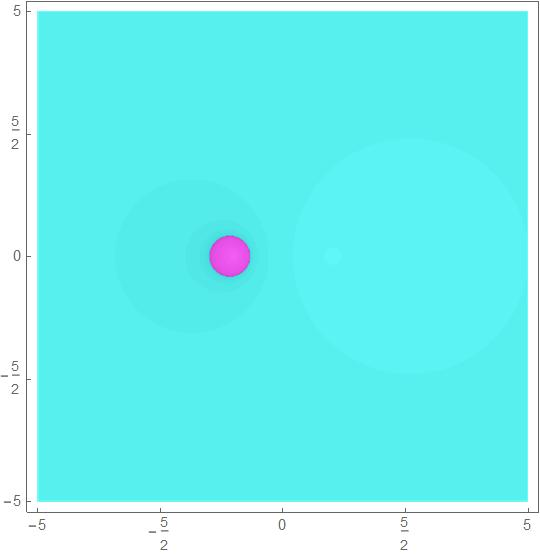
\includegraphics[width=0.98\textwidth]{fuentes/articulo-cuadraticos/imagenes/sch_m_5n_1.jpg}
\small Schröder: $m=5, \, n=1.$
\end{minipage}\hfill
\begin{minipage}[t]{0.45\textwidth}
\centering
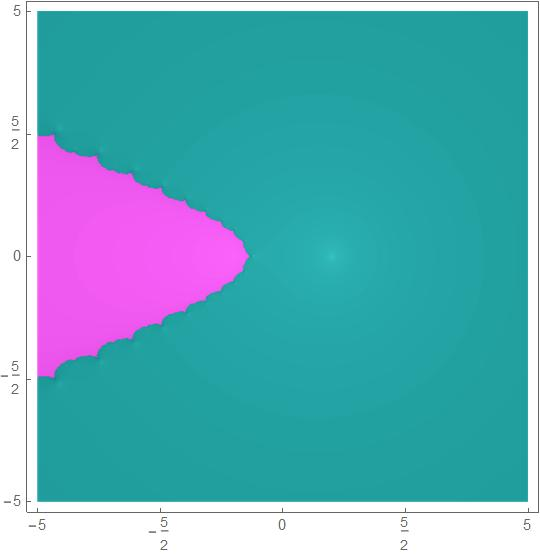
\includegraphics[width=0.98\textwidth]{fuentes/articulo-cuadraticos/imagenes/newton_m_5n_1.jpg}
\small Newton: $m=5, \, n=1.$
\end{minipage}

\vspace{0.5cm}

\begin{minipage}[t]{0.45\textwidth}
\centering
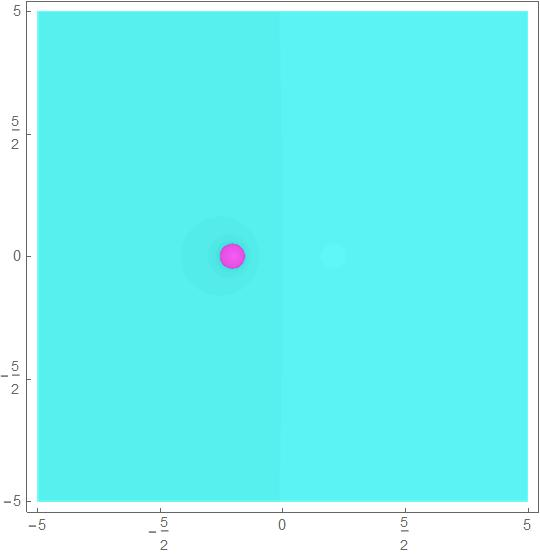
\includegraphics[width=0.98\textwidth]{fuentes/articulo-cuadraticos/imagenes/sch_m_8n_1.jpg}
\small Schröder: $m=8, \, n=1.$
\end{minipage}\hfill
\begin{minipage}[t]{0.45\textwidth}
\centering
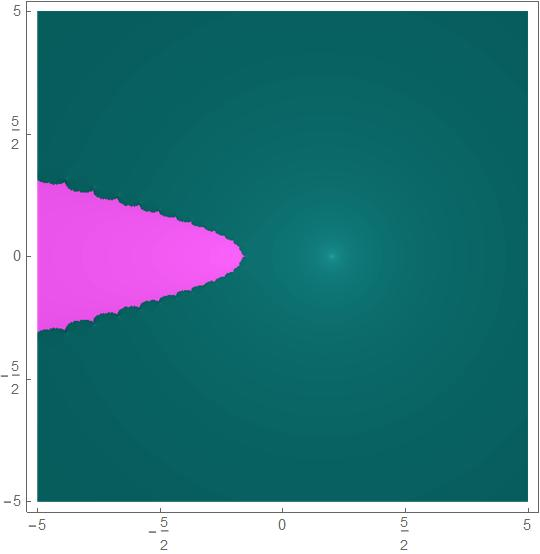
\includegraphics[width=0.98\textwidth]{fuentes/articulo-cuadraticos/imagenes/newton_m_8n_1.jpg}
\small Newton: $m=8, \, n=1.$
\end{minipage}

\caption{Cuencas de atracción de los métodos de Schröder y Newton aplicados a polinomios $(z-1)^m(z+1)^n$ para $n=1$ y $m=2, 5, 8$. Se aprecia cómo el conjunto de Julia del método de Schröder (un círculo) tiende a colapsar en la raíz $z=-1$ de menor multiplicidad. En el caso de Newton, el Julia es una ``parábola deformada'' cuyo vértice se aproxima también a $z=-1$ y cuyo ``ancho'' tiende a cero. La cuenca de la raíz múltiple $z=1$ invade progresivamente el plano.}
\label{fig:p_creciente}
\end{figure}

\subsubsection{Caso: $p=m/n$ próximo a 1}

En la Figura~\ref{fig:p_proximo1} se muestra qué ocurre cuando $p=m/n\approx 1$, es decir, cuando las multiplicidades son similares. Se consideran polinomios $(z-1)^m(z+1)^n$ con $n=6$ y $m=6, 7, 8$.

\begin{figure}[H]
\centering 
\begin{minipage}[t]{0.45\textwidth}
\centering
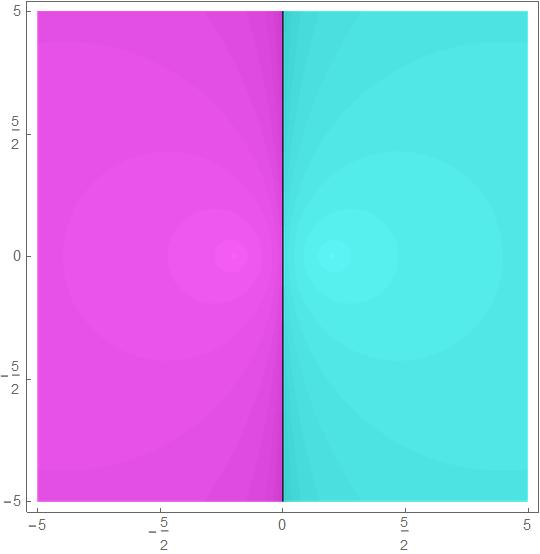
\includegraphics[width=0.98\textwidth]{fuentes/articulo-cuadraticos/imagenes/sch_n_6_m_6.jpg}
\small Schröder: $m=6, \, n=6.$
\end{minipage}\hfill
\begin{minipage}[t]{0.45\textwidth}
\centering
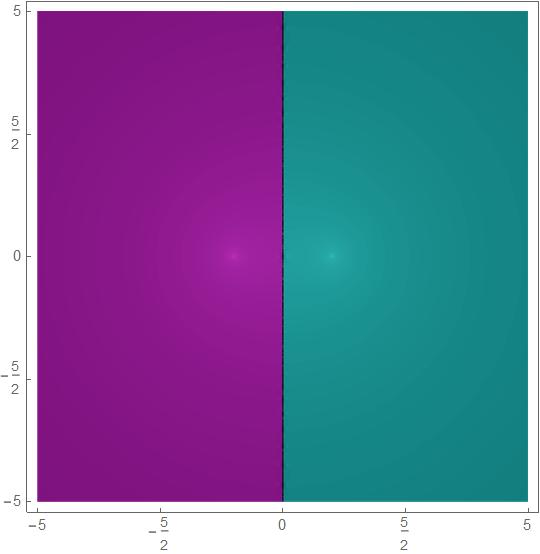
\includegraphics[width=0.98\textwidth]{fuentes/articulo-cuadraticos/imagenes/newton_n_6_m_6.jpg}
\small Newton: $m=6, \, n=6.$
\end{minipage}

\vspace{0.5cm}

\begin{minipage}[t]{0.45\textwidth}
\centering
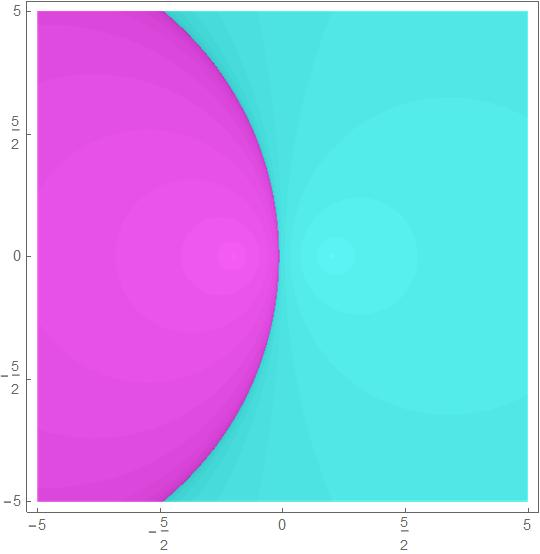
\includegraphics[width=0.98\textwidth]{fuentes/articulo-cuadraticos/imagenes/sch_m_7n_6.jpg}
\small Schröder: $m=7, \, n=6.$
\end{minipage}\hfill
\begin{minipage}[t]{0.45\textwidth}
\centering
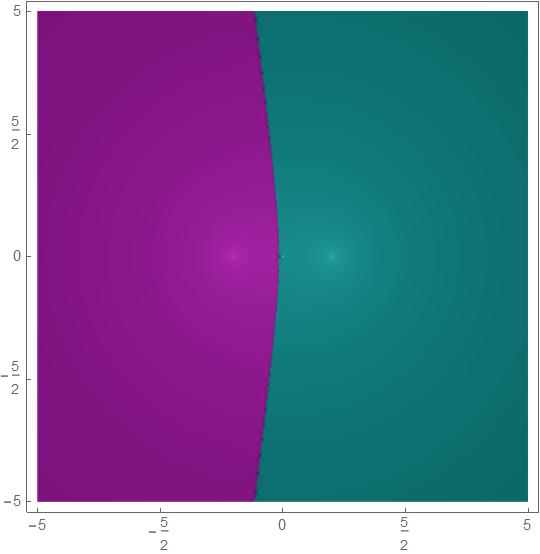
\includegraphics[width=0.98\textwidth]{fuentes/articulo-cuadraticos/imagenes/newton_m_7n_6.jpg}
\small Newton: $m=7, \, n=6.$
\end{minipage}

\vspace{0.5cm}

\begin{minipage}[t]{0.45\textwidth}
\centering
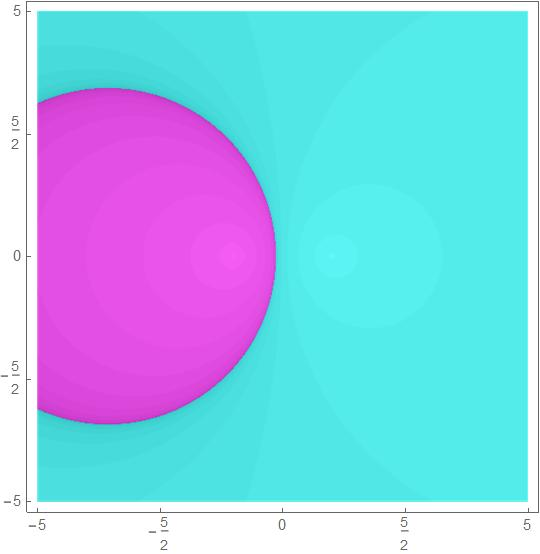
\includegraphics[width=0.98\textwidth]{fuentes/articulo-cuadraticos/imagenes/sch_m_8n_6.jpg}
\small Schröder: $m=8, \, n=6.$
\end{minipage}\hfill
\begin{minipage}[t]{0.45\textwidth}
\centering
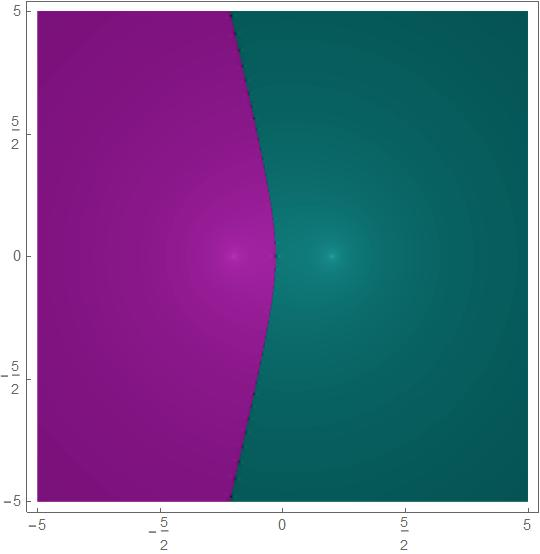
\includegraphics[width=0.98\textwidth]{fuentes/articulo-cuadraticos/imagenes/newton_m_8n_6.jpg}
\small Newton: $m=8, \, n=6.$
\end{minipage}

\caption{Cuencas de atracción de los métodos de Schröder y Newton aplicados a polinomios $(z-1)^m(z+1)^n$ para $n=6$ y $m=6, 7, 8$. El conjunto de Julia del método de Schröder son círculos que crecen a medida que $p$ se aproxima a 1, tendiendo a ``explotar'' en el eje imaginario cuando $p=1$ (caso $m=n=6$). Para Newton, la ``parábola deformada'' tiene su vértice cerca de $z=0$ y su ``ancho'' crece, tendiendo al eje imaginario cuando $p=1$.}
\label{fig:p_proximo1}
\end{figure}

\subsubsection{Caso: razón constante $p=2$}

La Figura~\ref{fig:p_constante} muestra el círculo correspondiente al conjunto de Julia del método de Schröder para polinomios con $p=m/n=2$, independientemente de los valores específicos de $m$ y $n$. También se aprecia que para Newton, aunque los valores absolutos de $m$ y $n$ influyen en la suavidad del Julia, la estructura general permanece similar para la misma razón $p$.

\begin{figure}[H]
\centering 
\begin{minipage}[t]{0.4\textwidth}
\centering
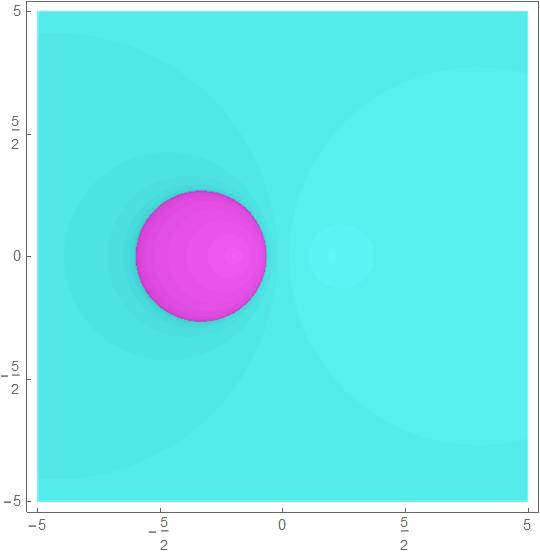
\includegraphics[width=0.88\textwidth]{fuentes/articulo-cuadraticos/imagenes/sch_m_4n_2.jpg}
\small Schröder: $p=m/n=2.$
\end{minipage}\hfill
\begin{minipage}[t]{0.4\textwidth}
\centering
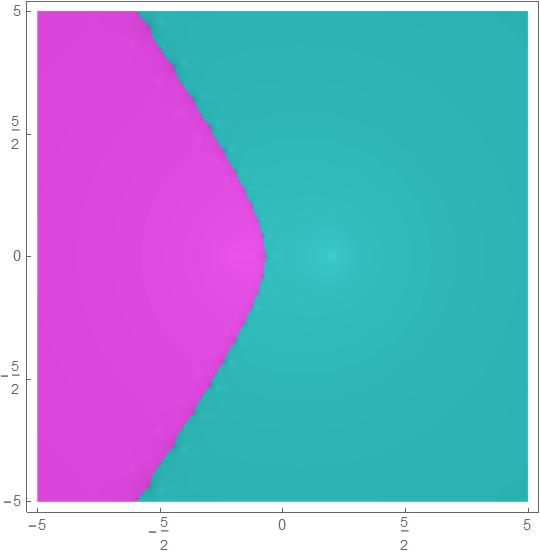
\includegraphics[width=0.88\textwidth]{fuentes/articulo-cuadraticos/imagenes/newton_m_4n_2.jpg}
\small Newton: $m=4, \, n=2.$
\end{minipage}

\vspace{0.5cm}

\begin{minipage}[t]{0.4\textwidth}
\centering
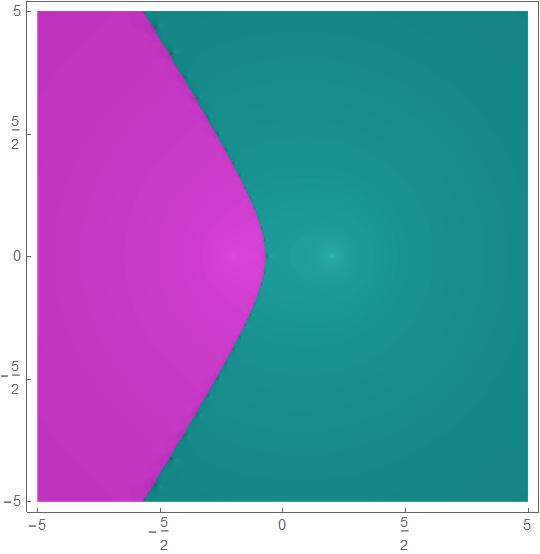
\includegraphics[width=0.88\textwidth]{fuentes/articulo-cuadraticos/imagenes/newton_m_6n_3.jpg}
\small Newton: $m=6, \, n=3.$
\end{minipage}\hfill
\begin{minipage}[t]{0.4\textwidth}
\centering
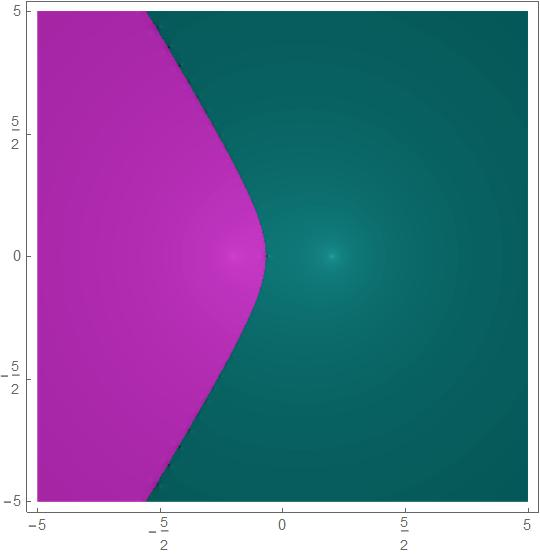
\includegraphics[width=0.88\textwidth]{fuentes/articulo-cuadraticos/imagenes/newton_m_8n_4.jpg}
\small Newton: $m=8, \, n=4.$
\end{minipage}

\caption{La primera imagen muestra la cuenca de atracción del método de Schröder aplicado a polinomios $(z-1)^m(z+1)^n$ con $p=m/n=2$. El conjunto de Julia es el mismo círculo para todos los pares $(m,n)$ con esta razón. Las otras imágenes muestran las cuencas del método de Newton para distintos valores de $m$ y $n$ con $p=m/n=2$. Se observa que la ``parábola deformada'' tiende a ser más suave conforme aumentan $m$ y $n$.}
\label{fig:p_constante}
\end{figure}

\subsubsection{Caso: raíces no reales}

Finalmente, en la Figura~\ref{fig:raices_complejas} se muestra un ejemplo con raíces no reales: $(z-1)^2(z-i)$. Se aprecia la pérdida de simetría respecto al eje imaginario, siendo ahora la recta equidistante entre las raíces la que juega el papel de eje de referencia.

\begin{figure}[H]
\centering 
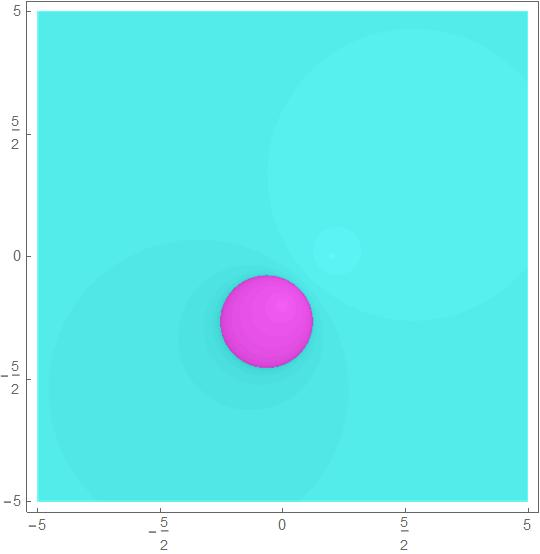
\includegraphics[width=0.4\textwidth]{fuentes/articulo-cuadraticos/imagenes/sch-i_m2_n1.jpg}\quad 
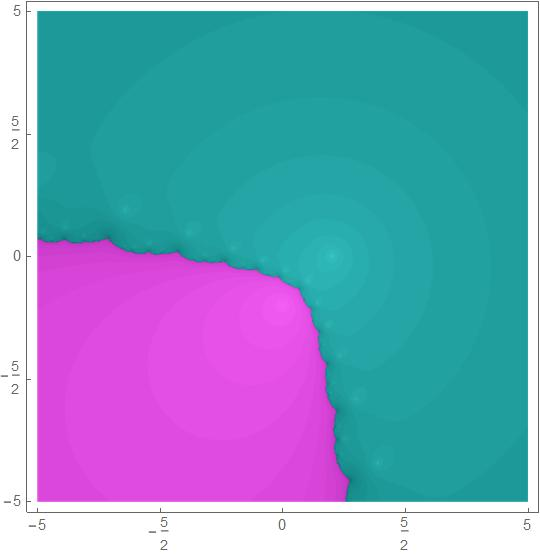
\includegraphics[width=0.4\textwidth]{fuentes/articulo-cuadraticos/imagenes/newton1-i_m2_n1.jpg}
\caption{Cuencas de atracción de los métodos de Schröder (izquierda) y Newton (derecha) aplicados al polinomio $(z-1)^2(z-i)$. El conjunto de Julia del método de Schröder sigue siendo un círculo dado por el Teorema~\ref{teo:julia_general}, pero ahora desplazado y sin la simetría respecto al eje imaginario. La frontera es ahora la perpendicular a la recta que une las raíces $z=1$ y $z=i$.}
\label{fig:raices_complejas}
\end{figure}

\subsection{Comparación con el método de Newton}

El análisis anterior permite establecer una comparación sistemática entre los métodos de Schröder y Newton para polinomios con dos raíces de multiplicidades arbitrarias.

\subsubsection{Naturaleza del conjunto de Julia}

\begin{itemize}
\item \textbf{Schröder:} El conjunto de Julia es siempre un círculo (o una recta en el caso límite $m=n$), cuya posición y radio están dados explícitamente por el Teorema~\ref{teo:julia_general}. Esta geometría simple facilita el análisis teórico y la predicción del comportamiento.

\item \textbf{Newton:} El conjunto de Julia tiene forma de ``parábola deformada'' cuya caracterización exacta es más compleja. Su forma depende no solo de la razón $p=m/n$ sino también de los valores absolutos de $m$ y $n$.
\end{itemize}

\subsubsection{Distribución de las cuencas de atracción}

\begin{itemize}
\item \textbf{Caso $m=n$:} Ambos métodos tienen el mismo conjunto de Julia (la bisectriz entre las raíces) y las mismas cuencas de atracción (los dos semiplanos correspondientes).

\item \textbf{Caso $m>n$:} 
\begin{itemize}
\item Para Schröder, la cuenca de la raíz de menor multiplicidad está completamente contenida en un disco, rodeada por la cuenca de la raíz de mayor multiplicidad.
\item Para Newton, la cuenca de la raíz de menor multiplicidad tiene una estructura más compleja en forma de franja acotada por la ``parábola deformada'', pero que se extiende hasta el infinito en ciertas direcciones.
\end{itemize}
\end{itemize}

\subsubsection{Coste computacional y orden de convergencia}

\begin{itemize}
\item \textbf{Newton:} Orden de convergencia 2 para raíces simples, lineal para raíces múltiples. Coste: 1 evaluación de $f$ y 1 de $f'$ por iteración.

\item \textbf{Schröder:} Orden de convergencia 2 incluso para raíces múltiples (ventaja importante). Coste: 1 evaluación de $f$, 1 de $f'$ y 1 de $f''$ por iteración (coste similar a métodos de orden 3 de la familia Chebyshev-Halley).
\end{itemize}

El método de Schröder resulta especialmente ventajoso cuando se sabe de antemano que existen raíces múltiples, ya que mantiene convergencia cuadrática sin necesidad de conocer la multiplicidad.

\section{Polinomios cúbicos: estudio del plano de parámetros}

Extendemos ahora el estudio a polinomios cúbicos con tres raíces distintas. Este caso presenta una complejidad considerablemente mayor y revela fenómenos dinámicos inesperados que no aparecen en el caso de dos raíces.

\subsection{Polinomios cúbicos con tres raíces simples}

Consideramos ahora polinomios de la forma
\begin{equation}
p(z)=(z-a)(z-b)(z-c), \quad a,b,c\in\C, \quad a\ne b\ne c.
\label{eq:poly_cubico}
\end{equation}

A diferencia del caso de dos raíces, donde las cuencas de atracción estaban delimitadas por círculos y rectas, en el caso cúbico aparecen estructuras fractales y regiones de no convergencia. En la Figura~\ref{fig:cuenca_cubica_1} se muestran las cuencas de atracción del polinomio $(z^2-1)(z-3-i)$.

\begin{figure}[H]
\centering 
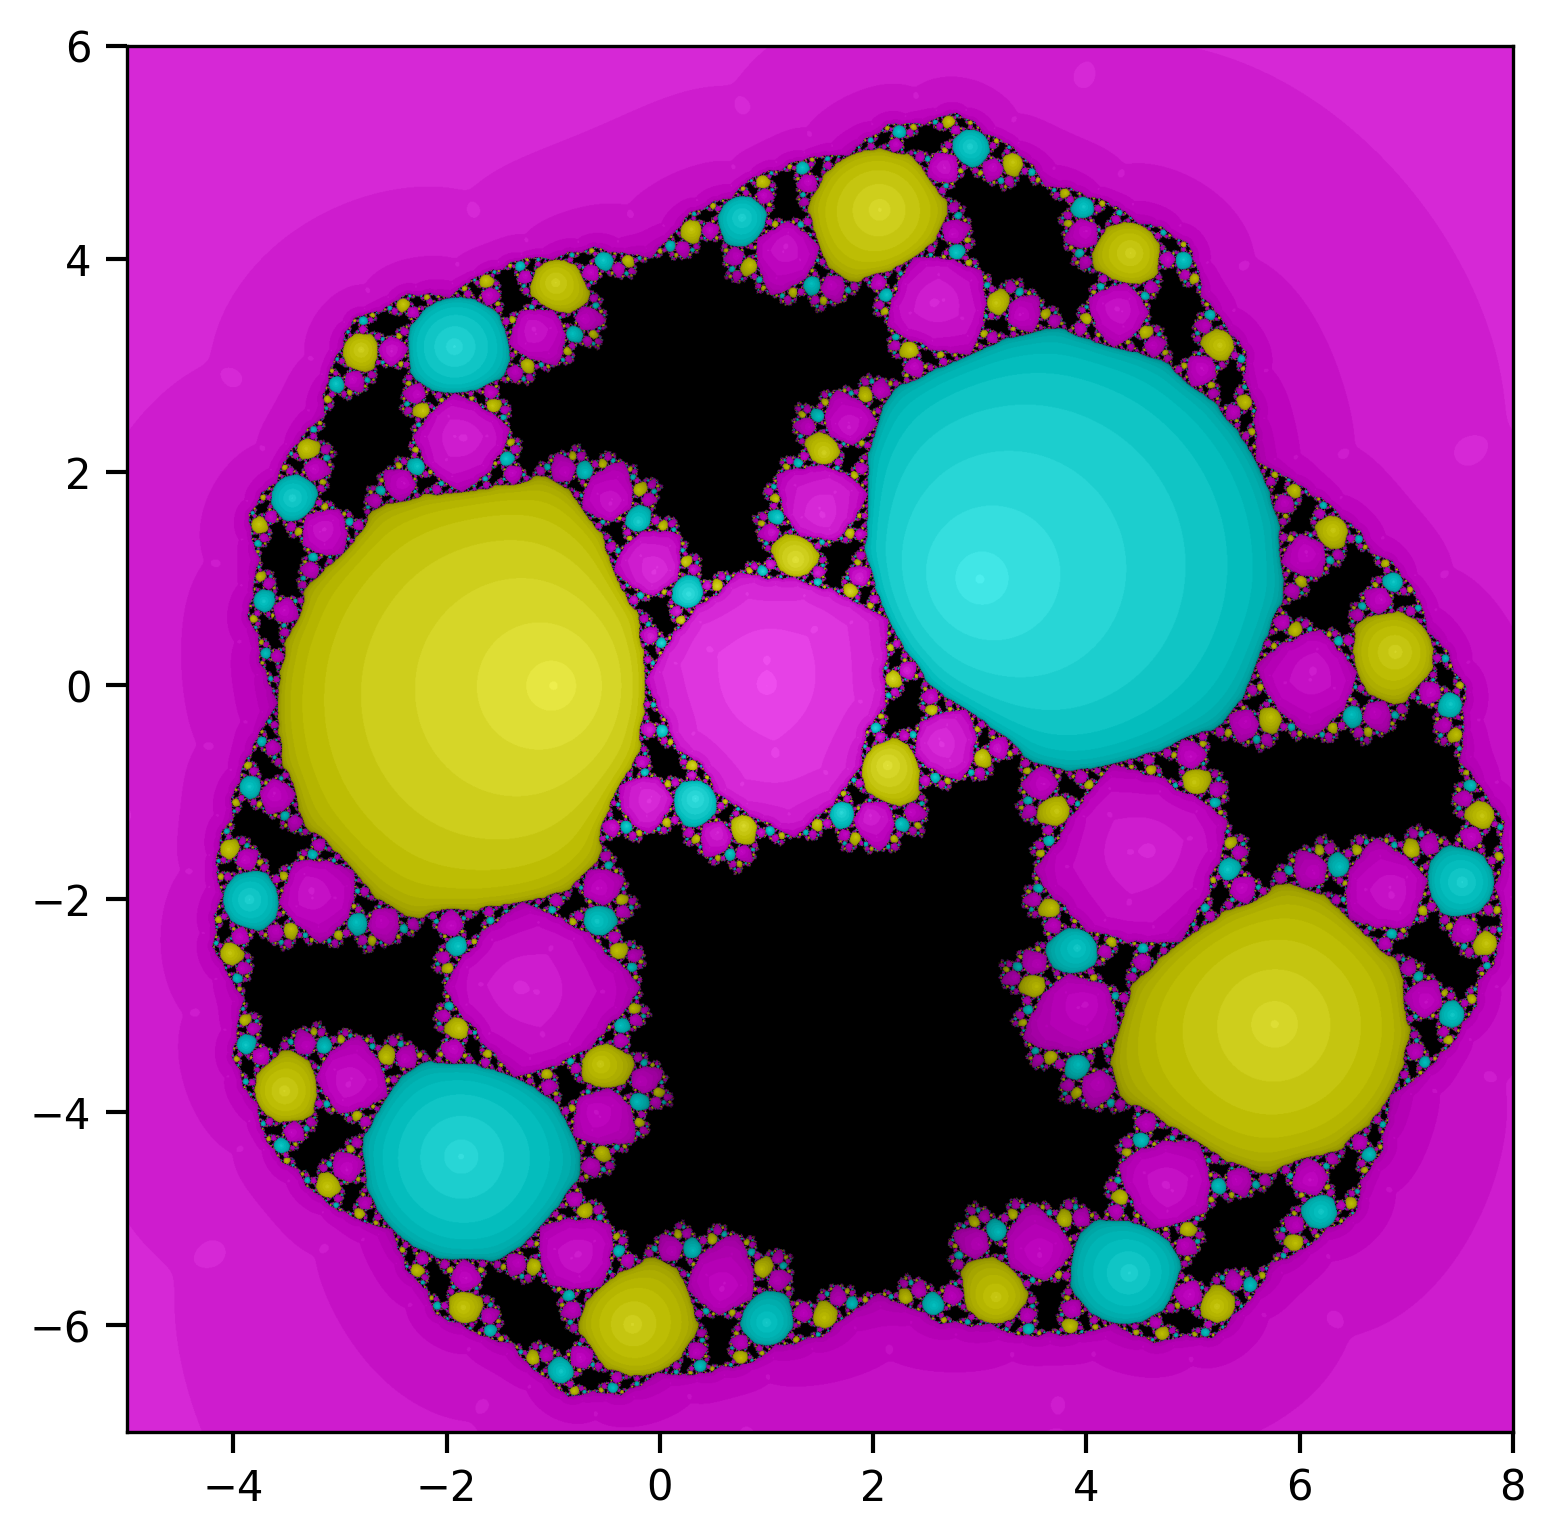
\includegraphics[width=0.6\textwidth]{img/sch_3+i.png}
\caption{Cuencas de atracción del método de Schröder aplicado a $p(z)=(z^2-1)(z-3-i)$. En cyan la cuenca de atracción de $z=1$, en magenta la de $z=-1$ y en amarillo la de $z=3+i$. Las zonas blancas representan puntos que no convergen a ninguna raíz tras un número determinado de iteraciones.}
\label{fig:cuenca_cubica_1}
\end{figure}

Observamos dos fenómenos importantes:
\begin{enumerate}
\item Existen regiones extensas (en negro) donde el método no converge a ninguna raíz.
\item La cuenca de atracción de la raíz $z=1$ (en cyan) domina ampliamente el plano, un comportamiento distinto al del método de Newton donde todas las cuencas se extienden hasta el infinito.
\end{enumerate}

\subsection{Puntos críticos y el teorema de Fatou-Julia}

Para entender el comportamiento observado, es fundamental analizar los puntos críticos de la función de iteración.

Un punto $\zeta\in\C$ se dice \textbf{punto crítico} de una función racional $R$ si la inyectividad de $R$ falla en un entorno de $\zeta$. Equivalentemente, $\zeta$ es punto crítico si $R'(\zeta)=0$ o si $R$ no está definida en $\zeta$.

\begin{teorema}[Teorema de Fatou-Julia]
\label{teo:fatou_julia}
Todo ciclo atractor de una función racional atrae al menos un punto crítico de ésta.
\end{teorema}

Este resultado es clave: las zonas blancas en la Figura~\ref{fig:cuenca_cubica_1} indican la presencia de ciclos atractores que no son las raíces del polinomio. Estos ciclos atraen alguno de los puntos críticos libres (aquellos que no son raíces).

\subsection{Reducción a una familia uniparamétrica}

Similar al análisis del caso cuadrático, podemos simplificar el estudio mediante una transformación afín.

\begin{teorema}
Sea $p(z)=(z-a)(z-b)(z-c)$ un polinomio cúbico con raíces distintas. Existe una transformación afín $A(z)=\alpha z+\beta$ tal que el polinomio transformado tiene la forma $q(z)=(z^2-1)(z-\lambda)$ con $\lambda\in\C$. Además, la función de iteración $S_p$ es conjugada a $S_q$ mediante $A$:
$$
A\circ S_q\circ A^{-1}=S_p.
$$
\end{teorema}

Los parámetros de la transformación están dados por:
$$
\alpha=\frac{a-b}{2}, \quad \beta=\frac{a+b}{2}, \quad \lambda=\frac{2c-a-b}{a-b}.
$$

Este resultado reduce el estudio dinámico de todos los polinomios cúbicos con tres raíces distintas al estudio de la familia uniparamétrica
$$
P_\lambda=\{(z^2-1)(z-\lambda), \quad \lambda\in\C\}.
$$

\subsection{Análisis de puntos críticos}

La función de iteración de Schröder para $p_\lambda(z)=(z^2-1)(z-\lambda)$ es:
$$
S_{p_\lambda}(z)=\frac{4\lambda^2 z+\lambda(z^4-10z^2+1)+4z^3}{2\lambda^2(z^2+1)-4\lambda(z^3+z)+3z^4+1}.
$$

Su derivada es:
$$
S'_{p_\lambda}(z)=-\frac{4(z^2-1)(z-\lambda)(-2\lambda^3-2\lambda+\lambda^2 z^3+3z^3-12\lambda z^2+9\lambda^2 z+3z)}{(2\lambda^2+3z^4-4\lambda z^3+2\lambda^2 z^2-4\lambda z+1)^2}.
$$

Las raíces $-1$, $1$ y $\lambda$ son puntos críticos que convergen a sí mismas. Los puntos críticos \emph{libres} son las raíces del numerador:
$$
-2\lambda^3-2\lambda+\lambda^2 z^3+3z^3-12\lambda z^2+9\lambda^2 z+3z=0.
$$

Esta ecuación cúbica en $z$ tiene tres soluciones $\zeta_1(\lambda)$, $\zeta_2(\lambda)$ y $\zeta_3(\lambda)$ (expresiones complejas que se pueden calcular explícitamente mediante las fórmulas de Cardano).

\subsection{El plano de parámetros}

Hay que entender el punto de que cuando al menos uno de los puntos críticos libres converja a algo diferente de una raíz, entonces  van a existir ciclos atractores para ese valor de $\lambda$

\begin{figure}[H]
\centering 
\begin{minipage}[t]{0.48\textwidth}
\centering
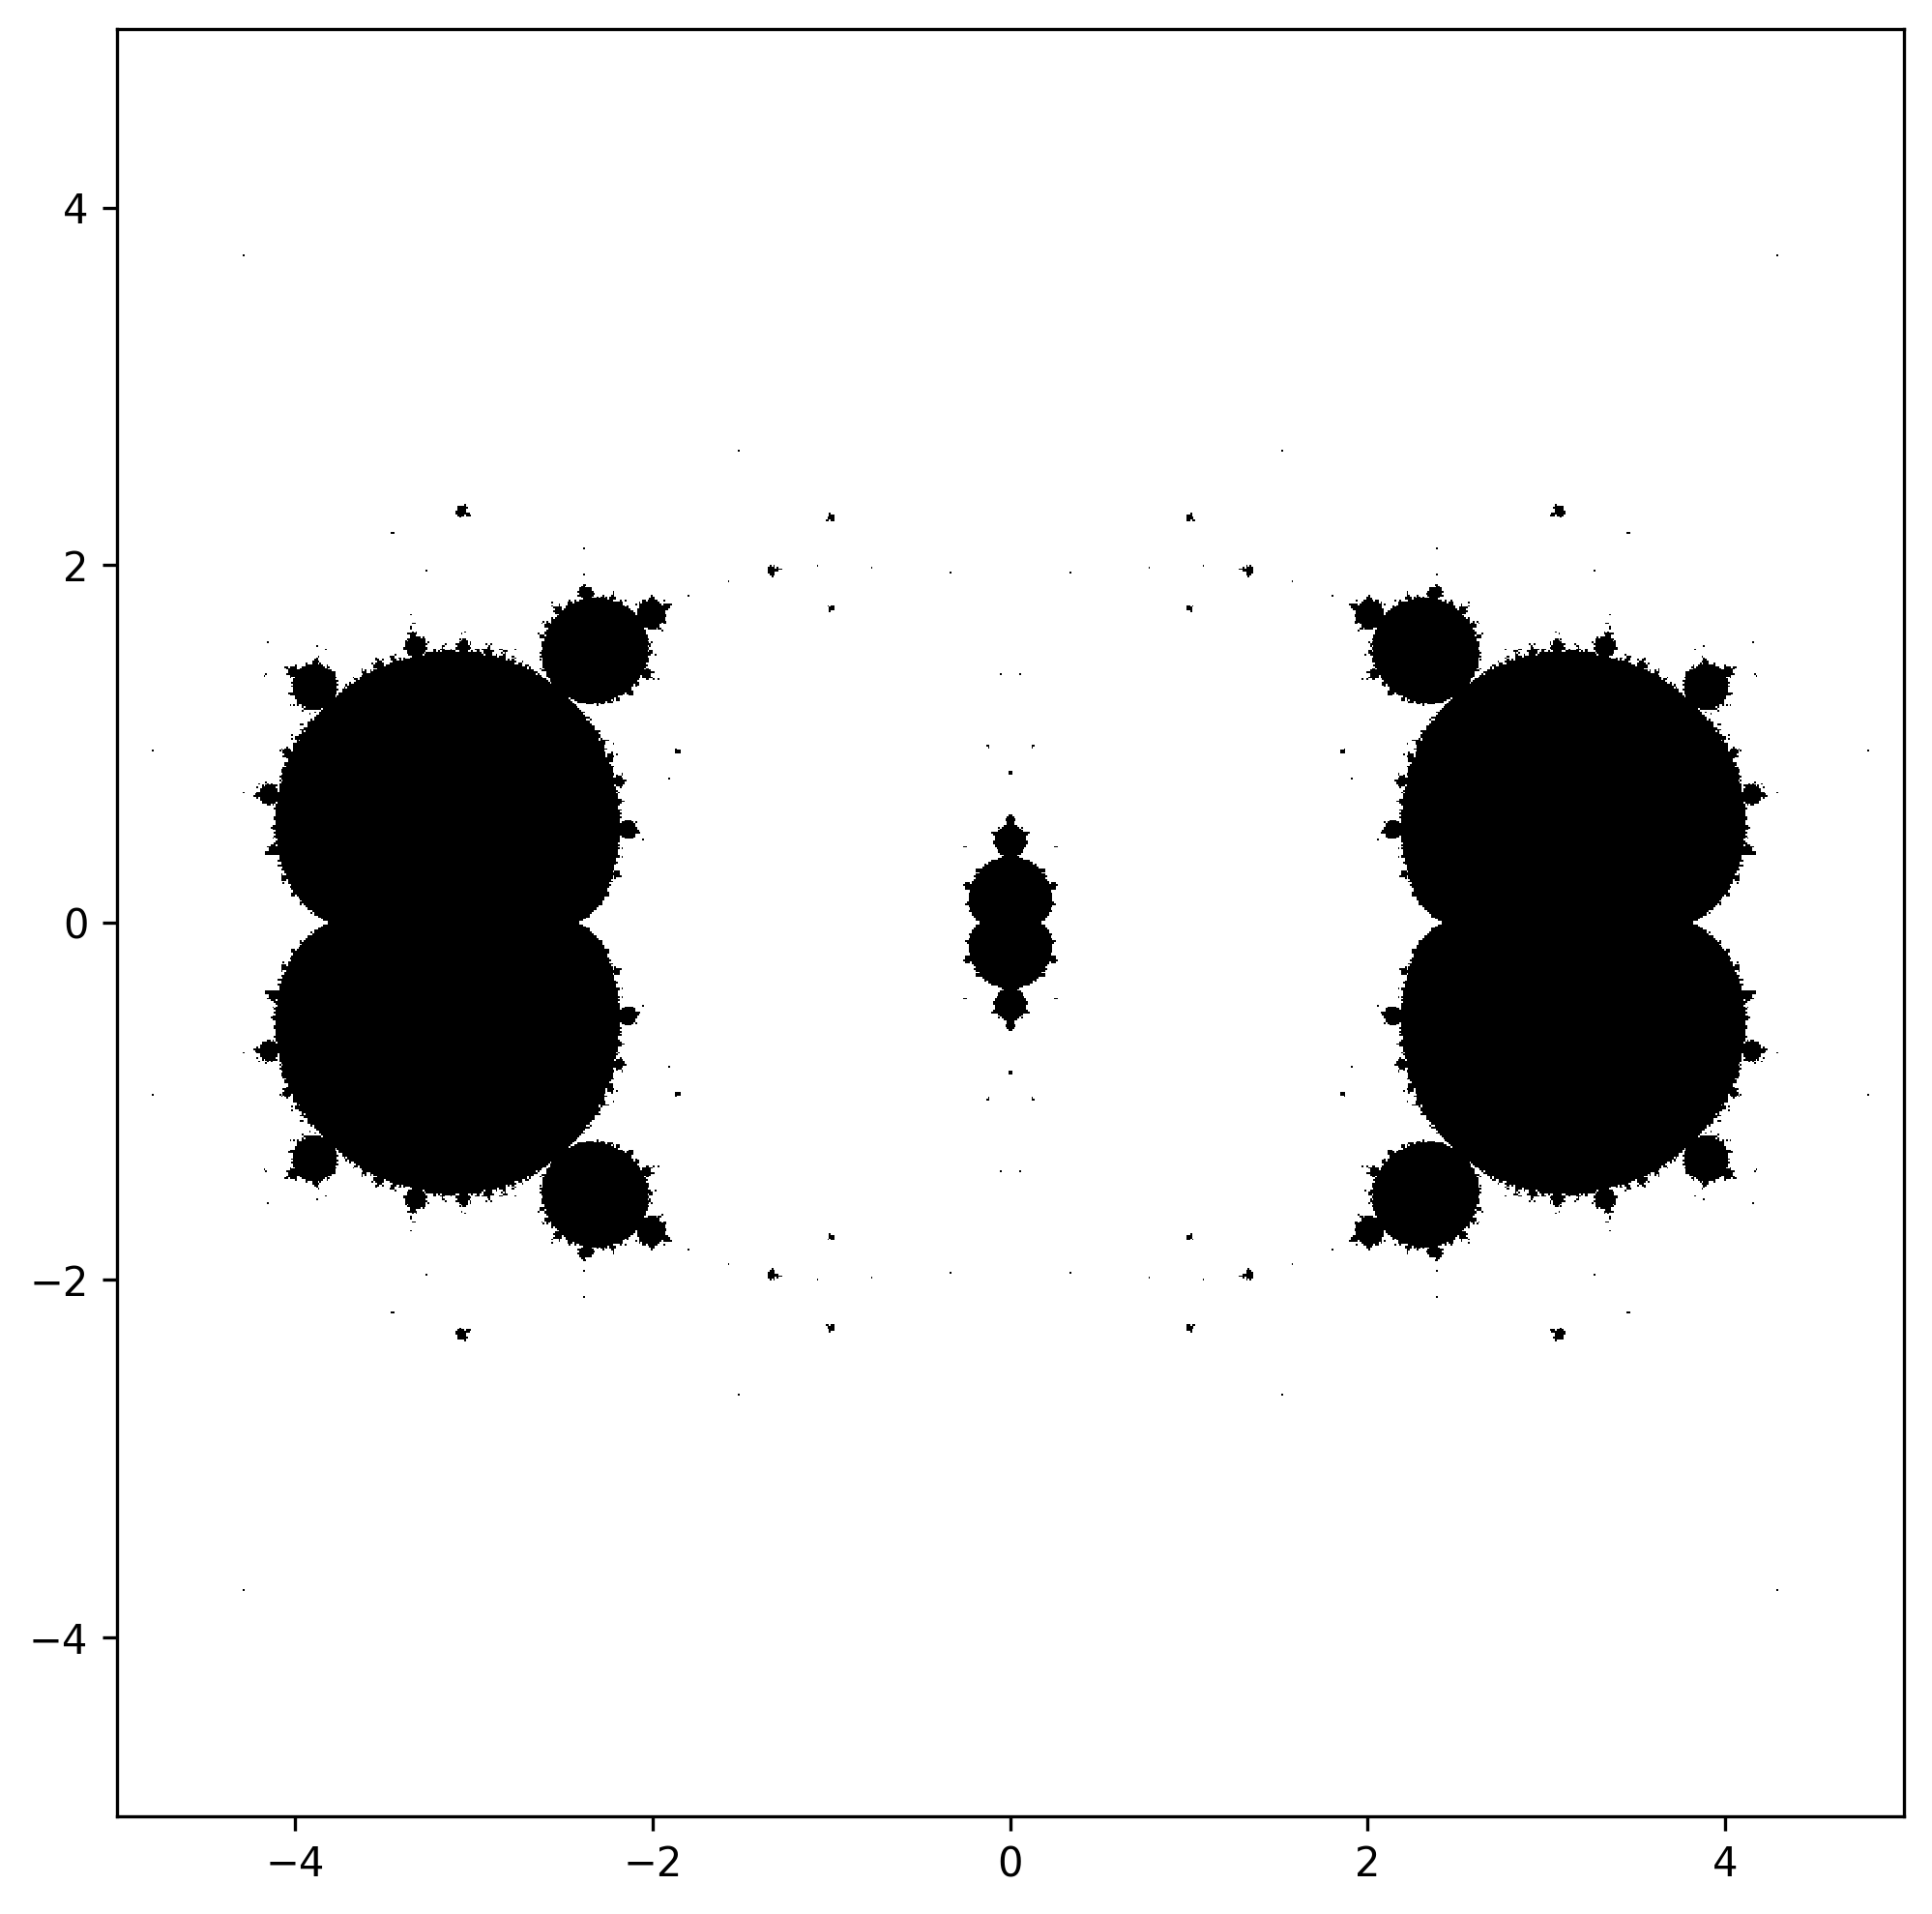
\includegraphics[width=\textwidth]{img/plano_param_sch_2.png}
\end{minipage}\hfill
\begin{minipage}[t]{0.48\textwidth}
\centering
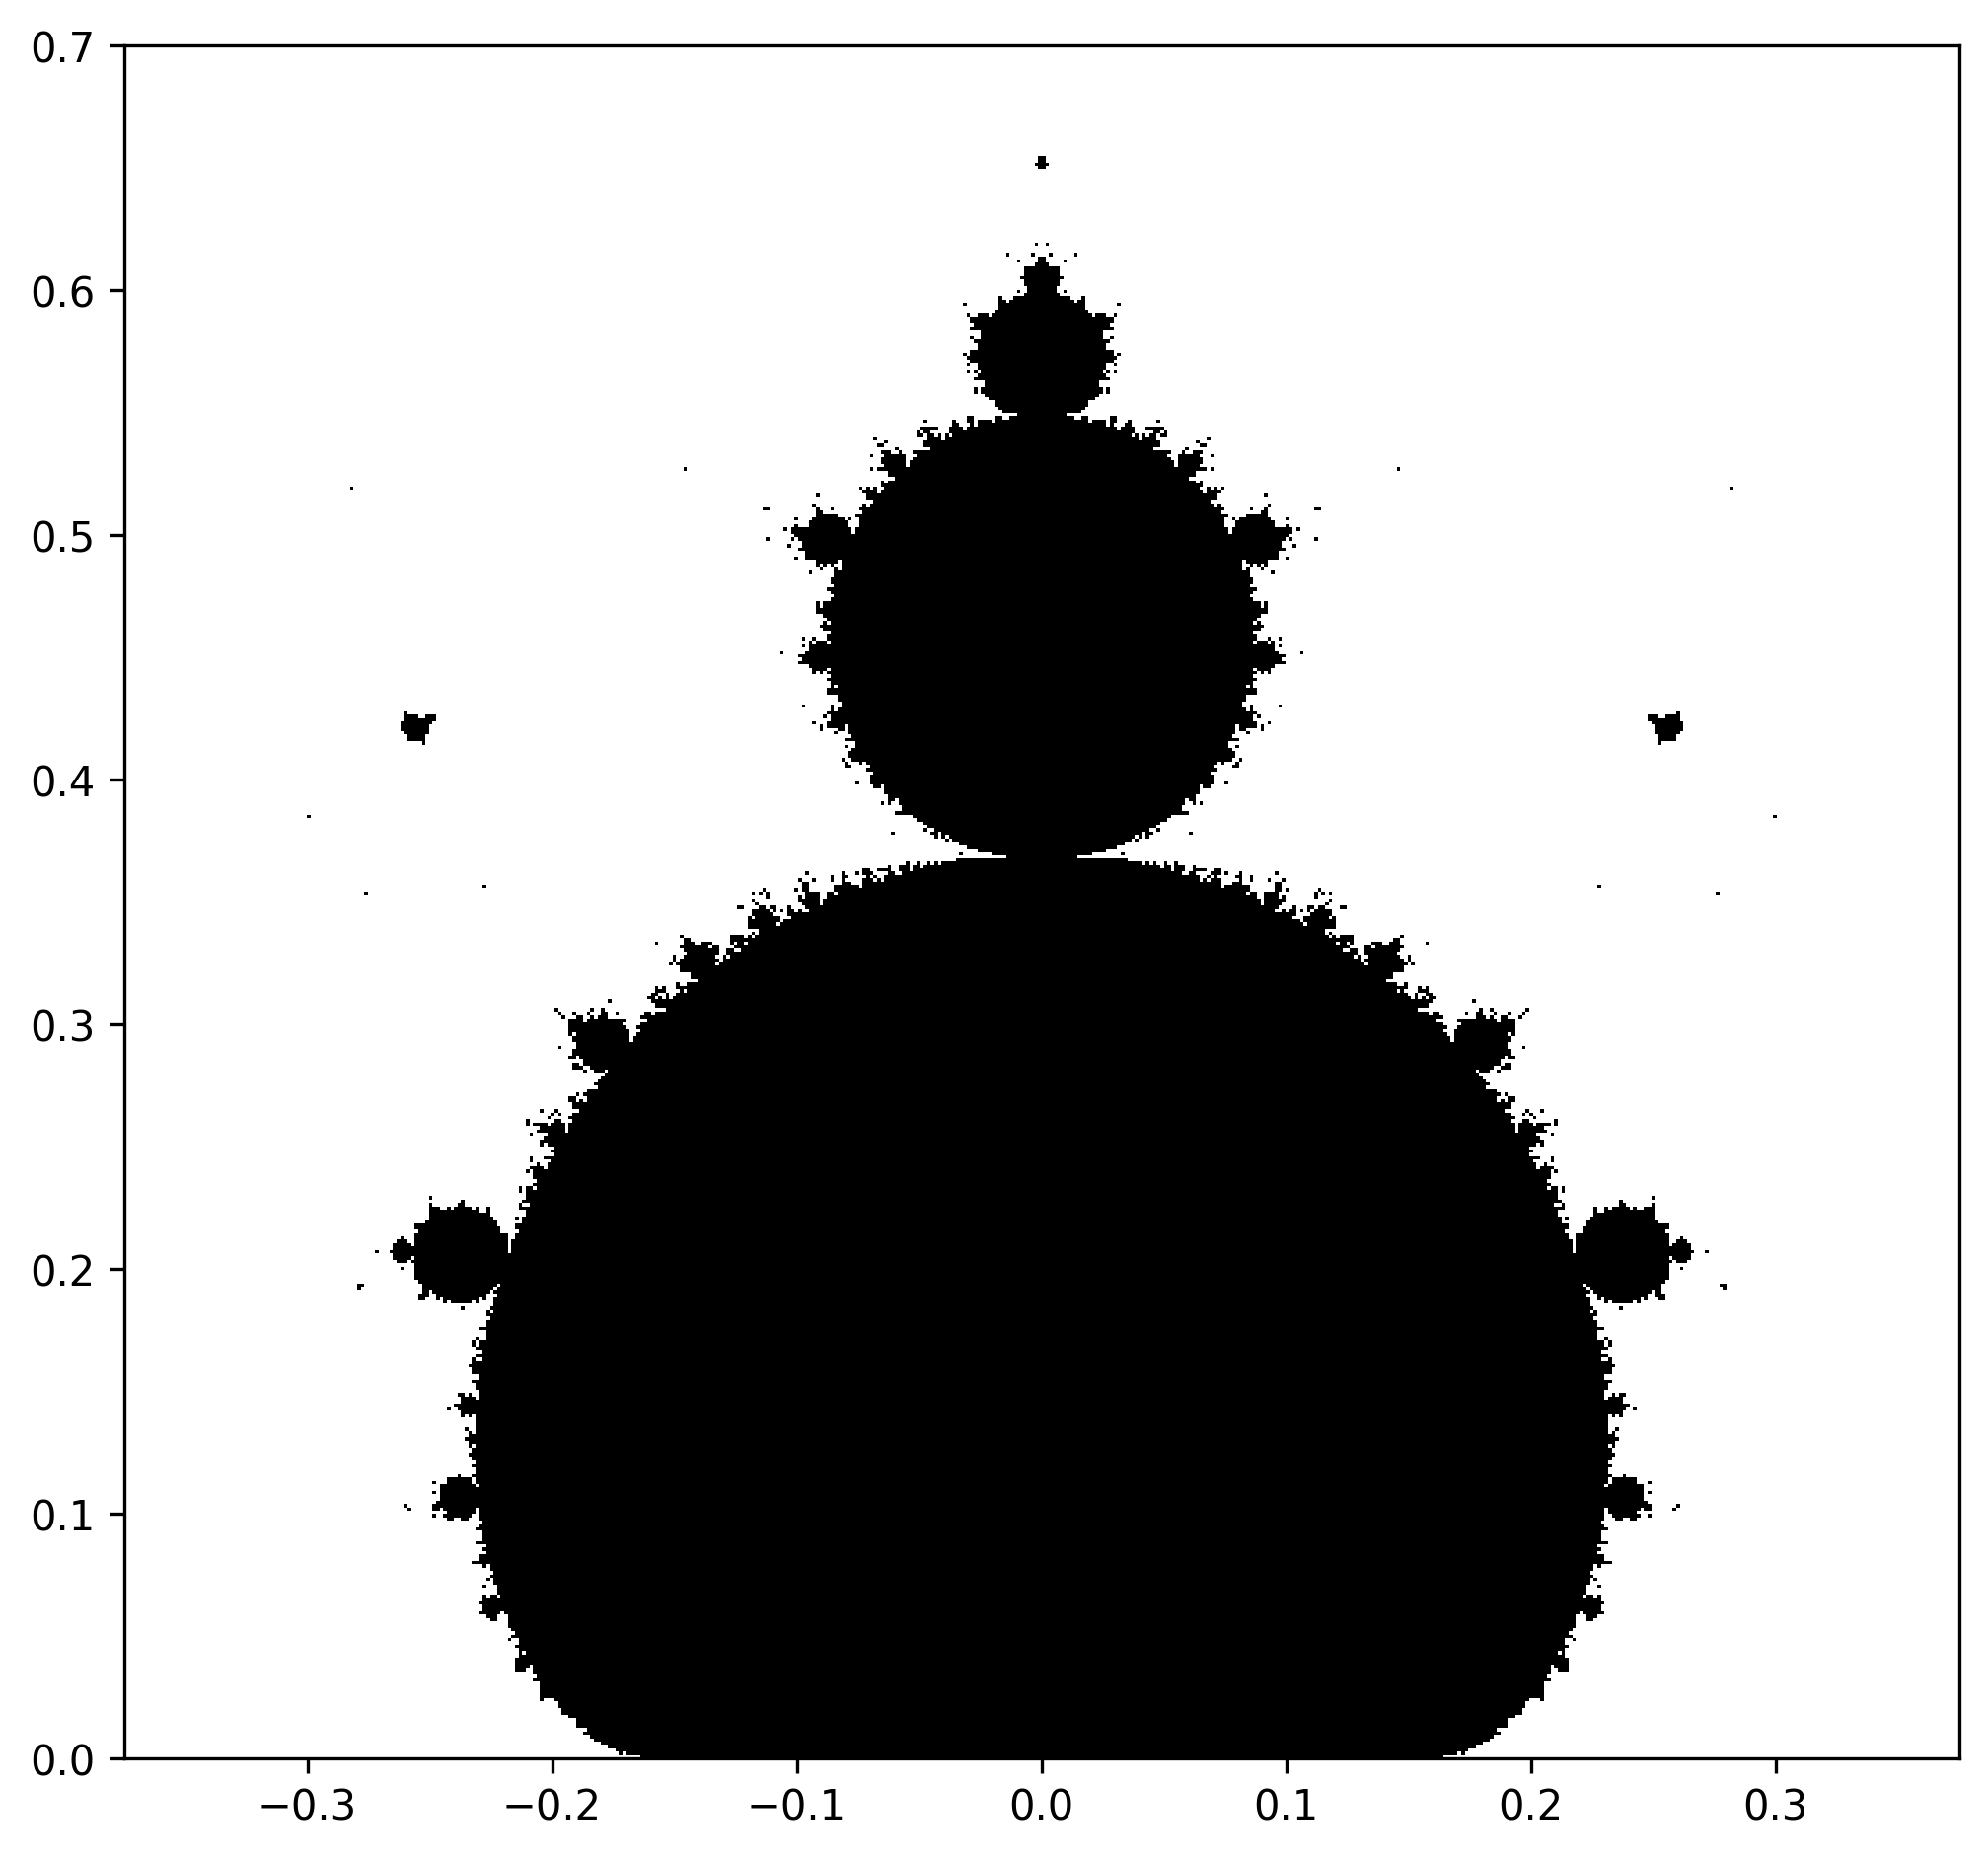
\includegraphics[width=\textwidth]{img/plano_param_sch_1.png}
\end{minipage}
\caption{Planos de parámetros del método de Schröder para los puntos críticos libres.}
\label{fig:planos_param_sch}
\end{figure}


Las zonas negras del plano de parámetros corresponden a valores de $\lambda$ para los cuales al menos un punto crítico libre asociado no converge a ninguna raíz, indicando la presencia de ciclos atractores adicionales.
Numéricamente se ha comprobado que si coges valores $\lambda$ de los sucesivos lóbulos autosemejantes del conjunto de tipo Mandelbrot central, se obtienen $2^n$ ciclos.


\subsection{Comparación con el método de Newton}

El método de Newton aplicado al mismo polinomio $p_\lambda(z)=(z^2-1)(z-\lambda)$ tiene función de iteración:
$$
N_{p_\lambda}(z)=\frac{-\lambda+2z^3-\lambda z^2}{3z^2-2\lambda z-1}.
$$

Su derivada es:
$$
N'_{p_\lambda}(z)=\frac{2(z^2-1)(z-\lambda)(3z-\lambda)}{(3z^2-2\lambda z-1)^2}.
$$

El método de Newton tiene un único punto crítico libre: $\zeta=\lambda/3$. Su plano de parámetros se muestra en la Figura~\ref{fig:plano_param_newton}.

\begin{figure}[H]
\centering 
\begin{minipage}[t]{0.48\textwidth}
\centering
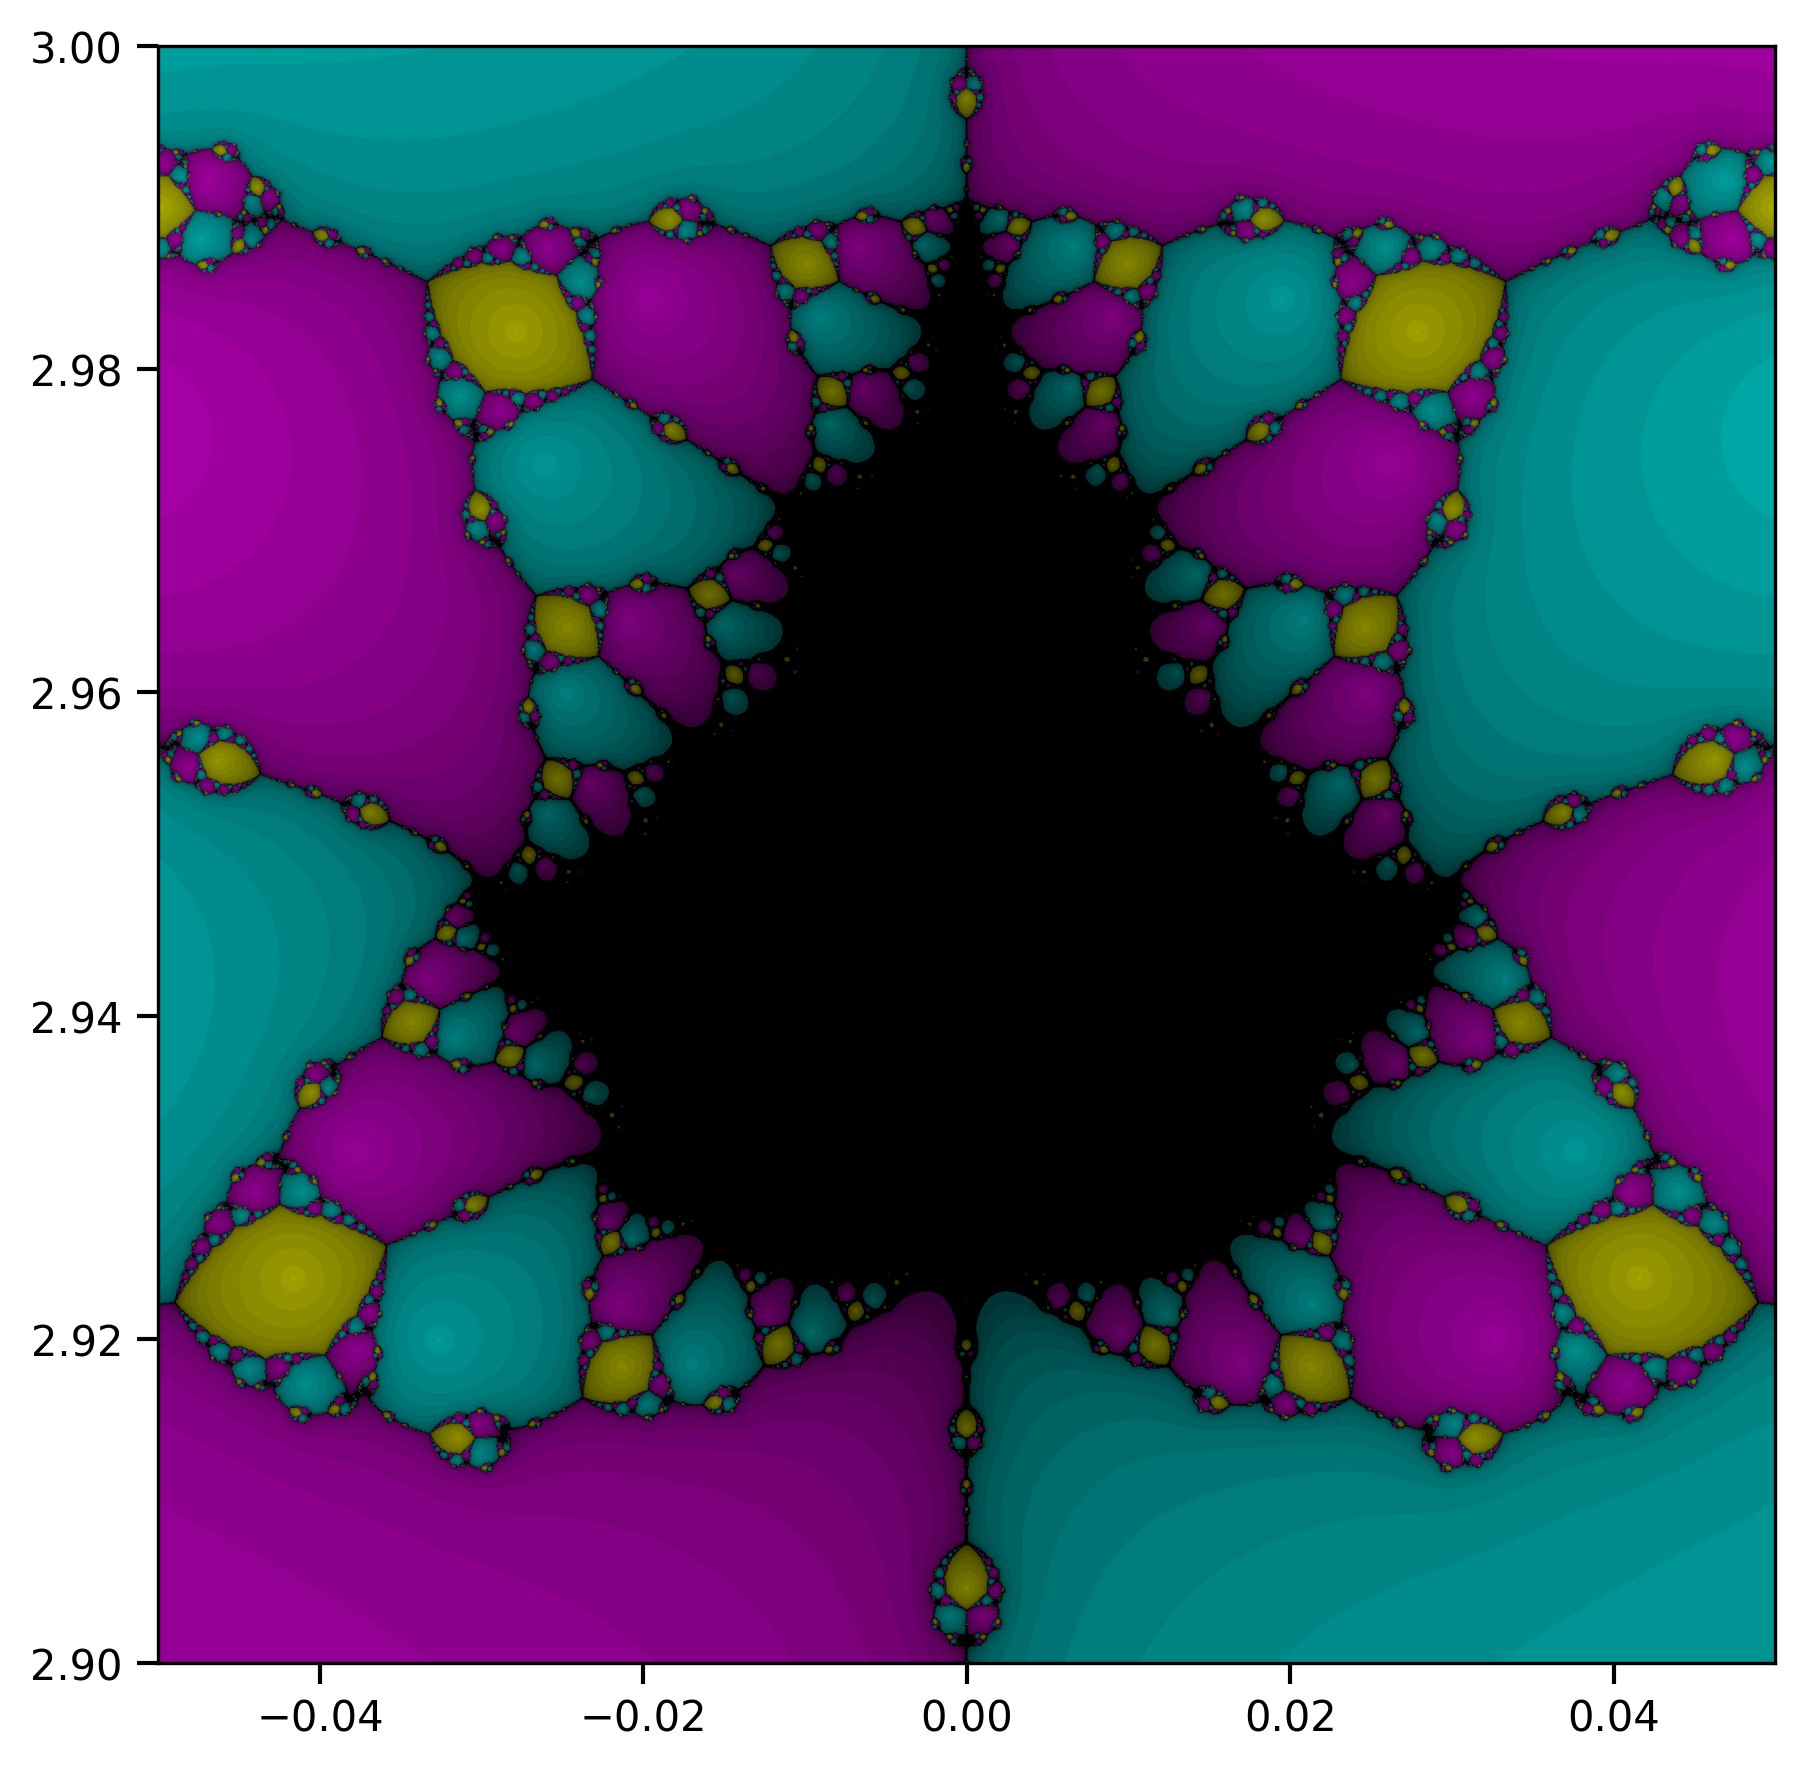
\includegraphics[width=\textwidth]{img/plan_param_newton_2.png}
\end{minipage}\hfill
\begin{minipage}[t]{0.48\textwidth}
\centering
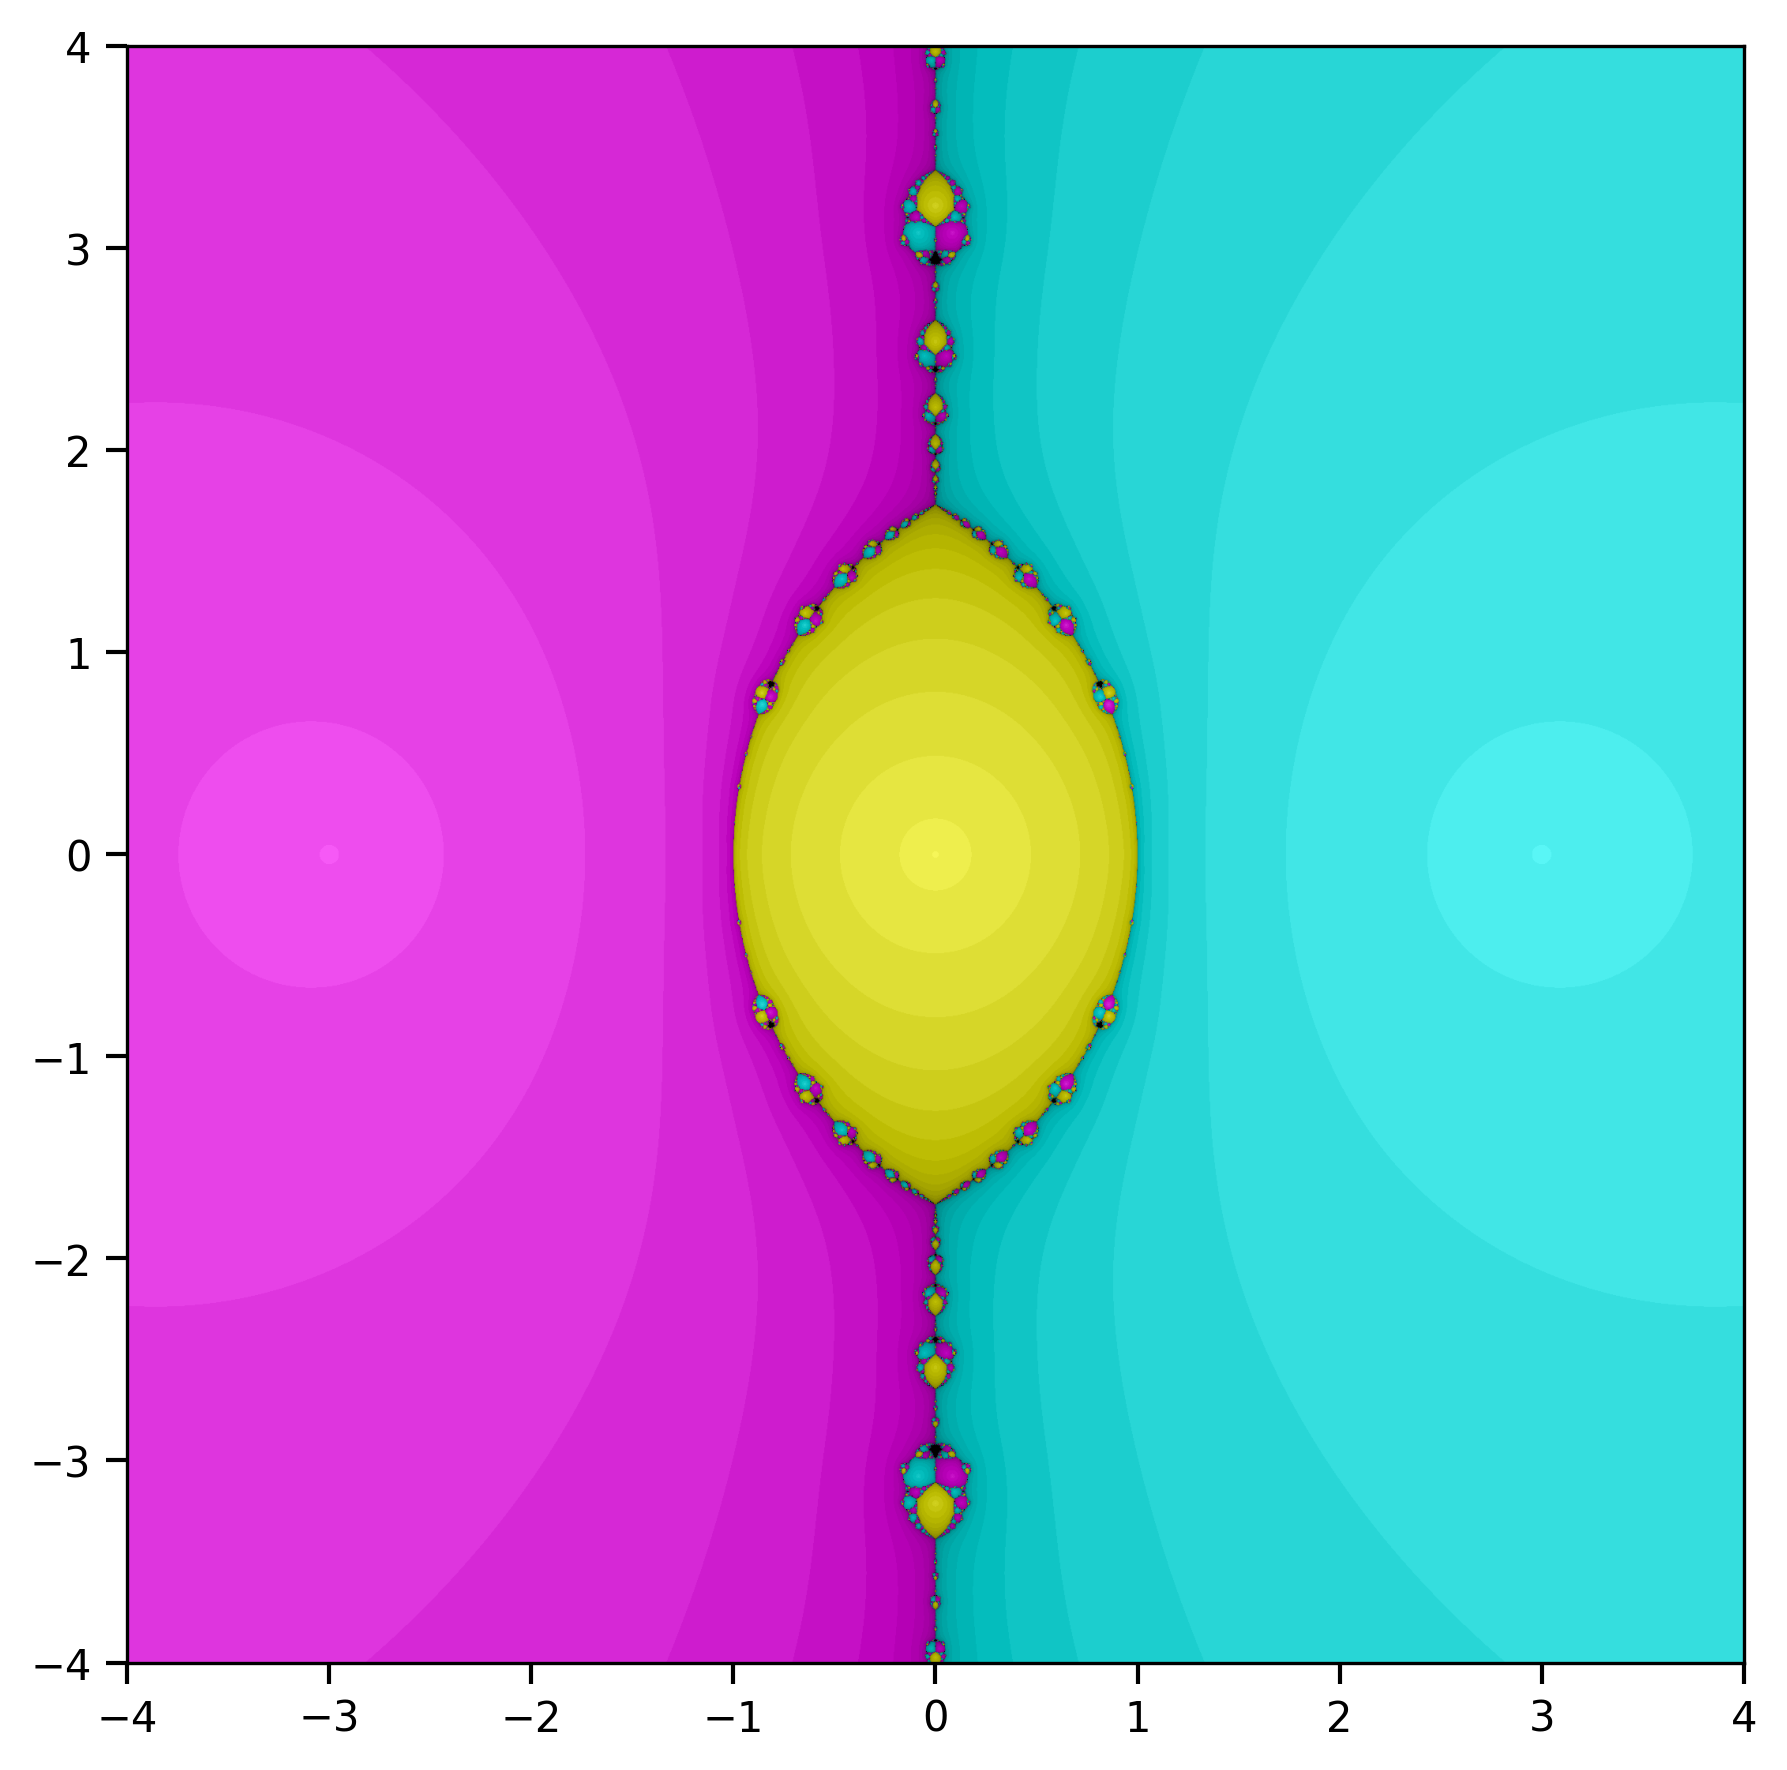
\includegraphics[width=\textwidth]{img/plan_param_newton_1.png}
\end{minipage}
\caption{Planos de parámetros del método de Schröder para los puntos críticos libres.}
\label{fig:planos_param_sch}
\end{figure}

Comparando con las Figuras~\ref{fig:plano_param_1}--\ref{fig:plano_param_3}, observamos que:
\begin{itemize}
\item Newton tiene un solo punto crítico libre, Schröder tiene tres.
\item Las zonas negras (no convergencia) son mucho más extensas en Schröder que en Newton.
\item La estructura del plano de parámetros es más simple para Newton.
\end{itemize}

\subsection{Caso especial: raíces formando un triángulo equilátero}

Un caso particularmente interesante ocurre cuando $\lambda=\sqrt{3}i$, pues las tres raíces $1$, $-1$ y $\sqrt{3}i$ forman un triángulo equilátero en el plano complejo.

Para este valor, la derivada de la función de iteración se simplifica a:
$$
S'_{p_{\sqrt{3}i}}(z)=-\frac{16(z-1)(z+1)(z-\sqrt{3}i)}{(3iz^3+3\sqrt{3}z^2-3iz+5\sqrt{3})^2}.
$$

En este caso, los únicos puntos críticos son las propias raíces. Por el Teorema~\ref{teo:fatou_julia}, no pueden existir ciclos atractores extraños, y por tanto todas las órbitas convergen a alguna de las tres raíces. Las cuencas de atracción para este caso se muestran en las Figuras~\ref{fig:cuenca_triangulo_1} y~\ref{fig:cuenca_triangulo_2}.

\begin{figure}[H]
\centering 
\begin{minipage}[b]{0.48\textwidth}
\centering
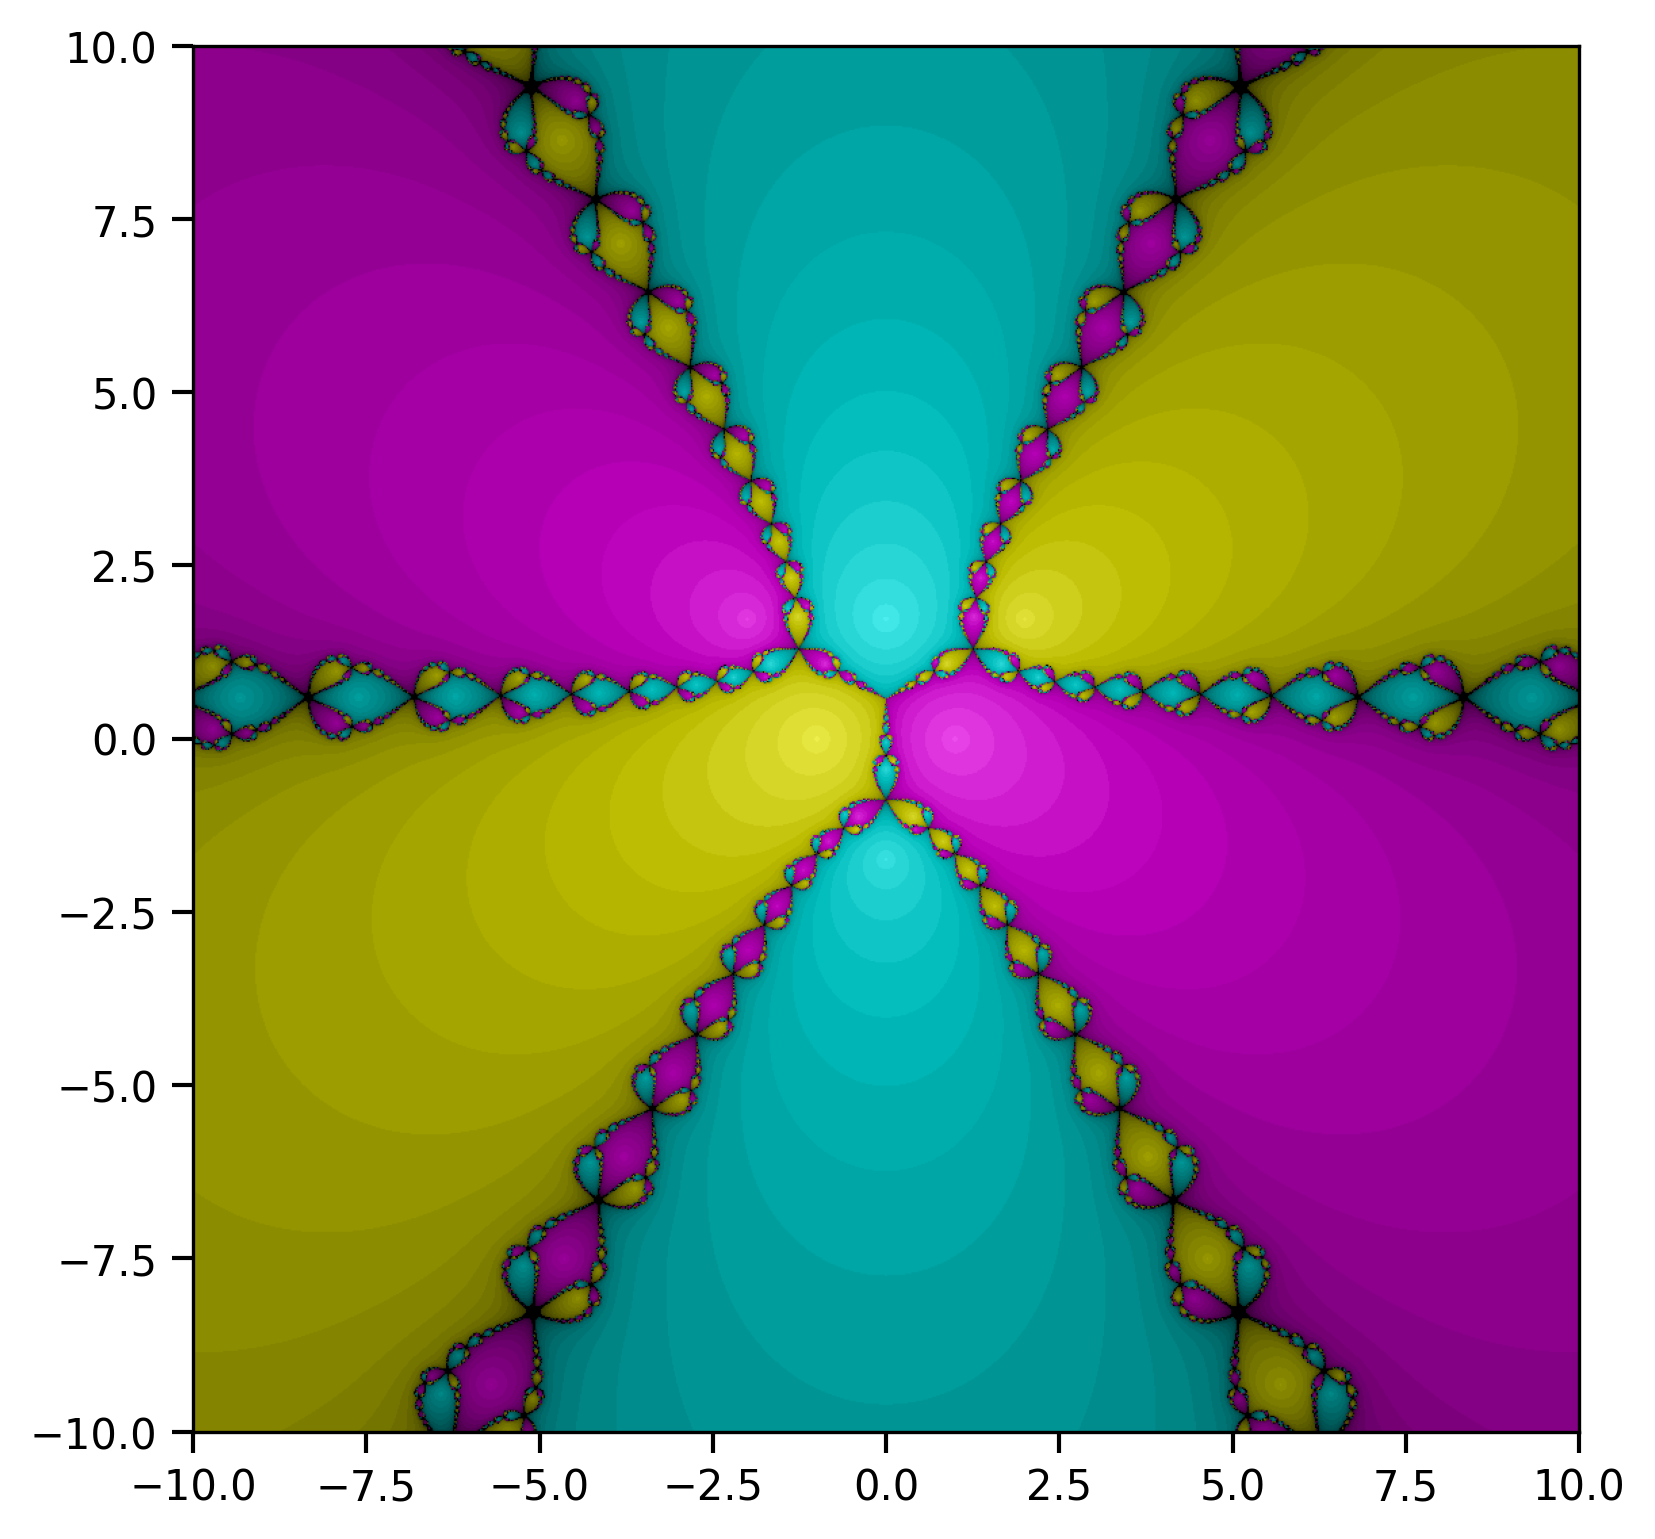
\includegraphics[width=\textwidth]{img/sch_sqrt3i_1.png}
\caption{Cuencas de atracción para $\lambda=\sqrt{3}i$ en la región $[-10,10]\times[-10i,10i]$.}
\label{fig:cuenca_triangulo_1}
\end{minipage}
\hfill
\begin{minipage}[b]{0.48\textwidth}
\centering
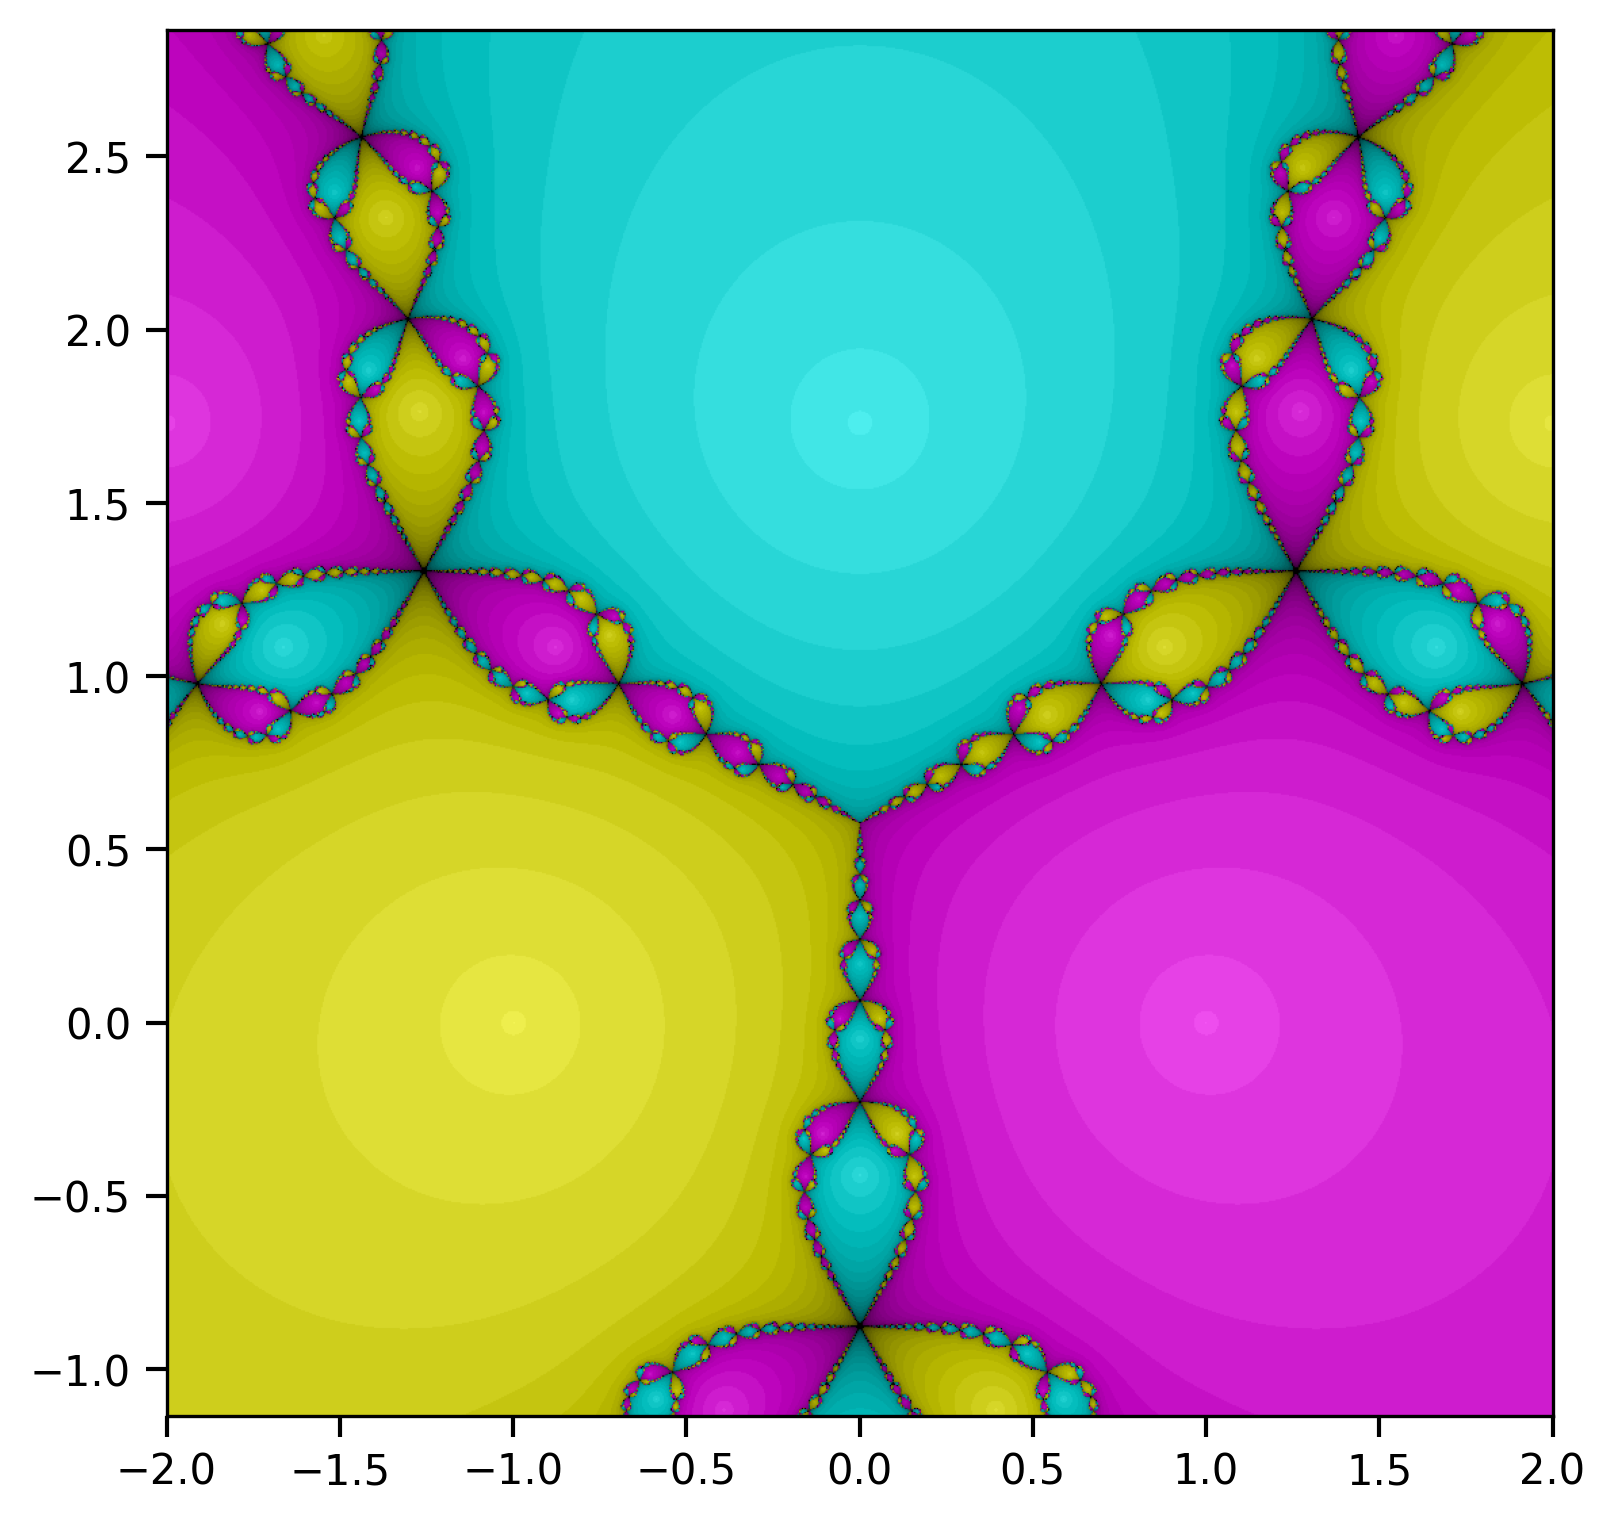
\includegraphics[width=\textwidth]{img/sch_sqrt3i_2.png}
\caption{Mismo caso en la región $[-2,2]\times[-2i,2i]$.}
\label{fig:cuenca_triangulo_2}
\end{minipage}
\end{figure}

\subsection{Observaciones dinámicas adicionales}

Los casos especiales analizados ($\lambda=\sqrt{3}i$ y $\lambda=0$) revelan la riqueza del espacio de parámetros. Mientras que para algunos valores de $\lambda$ todas las órbitas convergen a raíces (caso $\lambda=\sqrt{3}i$), para otros valores aparecen ciclos atractores que no son raíces (caso $\lambda=0$ con el 2-ciclo $\{i,-i\}$).

Este comportamiento contrasta notablemente con el caso de dos raíces, donde todos los puntos del plano complejo (excepto el conjunto de Julia) convergen necesariamente a una de las raíces. La presencia de tres puntos críticos libres en el caso cúbico, frente a ninguno en el caso de dos raíces, explica esta mayor complejidad dinámica.

% \section{Conclusiones}

% El estudio dinámico del método de Schröder en el plano complejo revela comportamientos cualitativamente distintos según el número de raíces del polinomio.

% \subsection{Síntesis de resultados para dos raíces}

% Para polinomios con dos raíces de multiplicidades arbitrarias:

% \begin{enumerate}
% \item El conjunto de Julia es siempre un círculo (o una recta cuando las multiplicidades son iguales), cuya ecuación explícita está dada por los Teoremas~\ref{teo:julia_canonico} y~\ref{teo:julia_general}.

% \item La razón $p=m/n$ entre multiplicidades es el parámetro fundamental que determina la geometría del Julia.

% \item Existe un comportamiento límite bien definido: colapso en la raíz simple cuando $p\to\infty$, y explosión en la bisectriz cuando $p\to 1^+$.

% \item La comparación con Newton muestra que Schröder tiene conjuntos de Julia más simples geométricamente (círculos vs. parábolas deformadas).

% \item El método de Schröder mantiene convergencia cuadrática para raíces múltiples, ventaja importante frente a Newton.
% \end{enumerate}

% \subsection{Síntesis de resultados para polinomios cúbicos}

% Para polinomios cúbicos con tres raíces simples:

% \begin{enumerate}
% \item La presencia de tres puntos críticos libres (frente a ninguno en el caso de dos raíces) introduce complejidad dinámica fundamental.

% \item Aparecen regiones extensas de no convergencia, correspondientes a ciclos atractores que no son raíces.

% \item El plano de parámetros revela una estructura compleja: para ciertos valores de $\lambda$ existen ciclos atractores extraños, mientras que para otros todas las órbitas convergen a raíces.

% \item El caso $\lambda=\sqrt{3}i$ (triángulo equilátero) es excepcional: no tiene puntos críticos libres y todas las órbitas convergen a alguna raíz.

% \item El caso $\lambda=0$ exhibe un 2-ciclo superatractor en $\{i,-i\}$, ilustrando claramente la existencia de atractores no triviales.

% \item El método de Newton, con un solo punto crítico libre, presenta un plano de parámetros más simple y menos zonas de no convergencia.
% \end{enumerate}

% \subsection{Implicaciones prácticas}

% Estos resultados tienen importantes implicaciones para el uso del método de Schröder:

% \begin{itemize}
% \item \textbf{Para polinomios con dos raíces:} El método es altamente predecible. La geometría circular del Julia facilita la selección de condiciones iniciales apropiadas. Es particularmente ventajoso en presencia de multiplicidades.

% \item \textbf{Para polinomios cúbicos:} La posible existencia de ciclos atractores extraños requiere precaución. El método puede no converger a ninguna raíz incluso con condiciones iniciales aparentemente razonables. Es recomendable implementar criterios de detección de no convergencia.

% \item \textbf{Comparación con Newton:} Mientras que Schröder supera a Newton en presencia de raíces múltiples, para polinomios con múltiples raíces simples, Newton puede ser más robusto debido a su menor número de puntos críticos libres.
% \end{itemize}

\section{El punto del infinito en el método de Schröder}

Una característica distintiva del método de Schröder, que lo diferencia de otros métodos iterativos como Newton, Halley o Chebyshev, es el comportamiento del punto del infinito. Mientras que en estos últimos métodos el infinito es un punto fijo repulsor, en el método de Schröder el infinito no es punto fijo, lo que introduce fenómenos dinámicos únicos que merecen un análisis detallado.

\subsection{Grado del método de Schröder}

En el estudio del comportamiento dinámico de métodos iterativos para resolver ecuaciones polinómicas, uno de los primeros pasos consiste en determinar el grado de la aplicación racional asociada. Si bien es relativamente sencillo establecer cotas superiores para este grado, el cálculo del valor exacto requiere la introducción del concepto de \emph{punto crítico especial}, tal como fue empleado por Nayak y Pal en su análisis de la aplicación racional asociada al método de Chebyshev.

\begin{definition}[Punto crítico especial]
Dado un polinomio complejo $p(z)$, un punto crítico $c\in\mathbb{C}$ se denomina especial si $p(c)\ne 0$ pero $p''(c) = 0$.
\end{definition}

Para mayor comodidad, escribimos la aplicación de iteración del método de Schröder de la forma equivalente
\begin{equation}
S_p(z)=z -\frac{p(z)p'(z)}{p'(z)^2- p(z)p''(z)}.
\label{eq:sch_alt_form}
\end{equation}

\begin{teorema}\label{teo:grado_schroder}
Sea $S_p(z)$ la aplicación de iteración del método de Schröder para resolver ecuaciones polinómicas, escrita como en \eqref{eq:sch_alt_form}. Entonces el grado de la aplicación racional $S_{p}(z)$ es
$$\deg(S_{p}(z)) =2r+s-C-2,$$
donde
\begin{itemize}
\item $r$ es el número de raíces distintas de $p(z)$.
\item $s$ es el número de puntos críticos especiales de $p(z)$.
\item $C=c_1+\cdots+c_k$ es la suma de multiplicidades de todos los puntos críticos especiales.
\end{itemize}
\end{teorema}

\begin{proof}
Comenzamos observando que $\deg(\text{Num}(S_p(z)))\le \deg(\text{Den}(S_p(z)))\le 2d-2$. En efecto, para un polinomio mónico general de la forma $p(z)=z^d +a_{d-1} z^{d-1} + \cdots$ es fácil demostrar, tras algunas manipulaciones algebraicas, que
$$ \text{Num}(S_p(z))=zp'(z)^2-zp(z)p''(z)-p(z)p'(z)=-a_{d-1}z^{2d-2}+P_{2d-3}(z), $$
$$ \text{Den}(S_p(z))=p'(z)^2-p(z)p''(z)=-dz^{2d-2}+Q_{2d-3}(z),$$
donde $P_{2d-3}(z)$ y $Q_{2d-3}(z)$ son polinomios de grado $2d-3$.

Consecuentemente, $\deg(S_p(z))\le 2d-2$. Además, $\deg(S_p(z))< 2d-2$ si $\text{Num}(S_p(z))$ y $\text{Den}(S_p(z))$ tienen raíces comunes. Para calcular el grado exacto de $S_p(z)$, debemos analizar $\deg(\text{Den}(S_p(z)))$.

La demostración se basa en las siguientes factorizaciones de los polinomios $p(z)$, $p'(z)$ y $p''(z)$:
\[
p(z)=\prod_{i=1}^m(z-\alpha_i)\prod_{j=1}^n(z-\beta_j)^{b_j},\quad b_j\ge 2,
\]
con $\deg(p)=m+B$, $B=\sum_{j=1}^n b_j.$ Teniendo en cuenta que una raíz de $p(z)$ con multiplicidad $k\ge 1$ es raíz de $p'(z)$ con multiplicidad $k-1$ (y un criterio similar para $p''(z)$), tenemos
$$p'(z)=g(z)\prod_{j=1}^n(z-\beta_j)^{b_j-1},$$
$$p''(z)=h(z)\prod_{j=1}^n(z-\beta_j)^{b_j-2},$$
donde $g(z)$ y $h(z)$ son polinomios que satisfacen $g(\alpha_i)\ne 0$, $i=1,\dots, m$, $g(\beta_j)\ne0$ y $h(\beta_j)\ne 0$ para $j=1,\dots, n$.

Además, $\deg(g)=\deg(p')-B+n=m+n-1$ y el coeficiente líder de $g(z)$ es $d$; $\deg(h)=\deg(p'')-B+2n=m+2n-2$ y el coeficiente líder de $h(z)$ es $d(d-1)$.

Sean $\gamma_j$, $j=1,\dots, s$ los puntos críticos especiales de $p(z)$, con multiplicidades $c_j$. Entonces los polinomios $g(z)$ y $h(z)$ pueden factorizarse de la siguiente manera:
$$g(z)=\tilde{g}(z)\prod_{k=1}^s(z-\gamma_k)^{c_k},$$
$$h(z)=\tilde{h}(z)\prod_{k=1}^s(z-\gamma_k)^{c_k-1},$$
donde $\tilde{g}(z)$ y $\tilde{h}(z)$ son polinomios que satisfacen $\tilde{g}(\alpha_i)\ne 0$, $i=1,\dots, m$; $\tilde{g}(\beta_j)\ne0$ y $\tilde{h}(\beta_j)\ne 0$ para $j=1,\dots, n$; $\tilde{h}(\gamma_k)\ne 0$ para $k=1,\dots, s$.

Además, $\deg(\tilde{g})=\deg(g)-C=m+n-C-1$ y el coeficiente líder de $\tilde{g}(z)$ es $d$; $\deg(\tilde{h})=\deg(h)-C+s=m+2n-2-C+s$ y el coeficiente líder de $h(z)$ es $d(d-1)$.

Por tanto, podemos simplificar las raíces comunes en el siguiente cociente
$$
\frac{p(z)p'(z)}{p'(z)^2- p(z)p''(z)}=\dfrac{\prod_{i=1}^m(z-\alpha_i)\prod_{j=1}^n(z-\beta_j) \prod_{k=1}^s(z-\gamma_k) \tilde{g}(z)}
{\prod_{k=1}^s(z-\gamma_k)^{(c_k+1)} \tilde{g}(z)^2-\prod_{i=1}^m(z-\alpha_i)\tilde{h}(z)}.
$$

El grado de $S_p(z)$ coincide con el denominador del cociente anterior (nótese que no hay más raíces comunes entre el numerador y el denominador de $S_p(z)$). El coeficiente líder del polinomio en el denominador del cociente anterior
$$
\prod_{k=1}^s(z-\gamma_k)^{(c_k+1)} \tilde{g}(z)^2-\prod_{i=1}^m(z-\alpha_i)\tilde{h}(z)
$$
es $d^2-d(d-1)=d$, y su grado es
$2m+2n+s-C-2 =2r+s-C-2$, siendo $r=m+n$ el número de raíces distintas de $p(z)$. Así queda demostrado el resultado.
\end{proof}

\begin{corolario}\label{cor:grado_sin_criticos}
Si $p(z)$ es un polinomio sin puntos críticos especiales, entonces el grado de la aplicación racional $S_{p}(z)$ es
$$\deg(S_{p}(z))=2r-2,$$
donde $r$ es el número de raíces distintas de $p(z)$.
\end{corolario}

Teniendo en cuenta la demostración del Teorema~\ref{teo:grado_schroder}, podemos caracterizar el comportamiento del punto del infinito para el método de Schröder. Como veremos, este comportamiento es diferente al de los procesos iterativos más conocidos (Newton, Halley y Chebyshev), para los cuales el infinito es un punto fijo repulsor.

\begin{corolario}\label{cor:infinito_no_fijo}
El punto en el infinito no es un punto fijo para el método de Schröder.
\end{corolario}

\begin{proof}
Siguiendo la demostración del Teorema~\ref{teo:grado_schroder}, y con las mismas notaciones, tenemos
$$
S_p(\infty)=-\frac{a_{d-1}}{d},
$$
por lo que $\infty$ no es un punto fijo para $S_p(z)$.
\end{proof}

Este resultado fundamental establece una diferencia crucial entre el método de Schröder y otros métodos iterativos clásicos, y motiva el estudio detallado del comportamiento del infinito que desarrollamos en las subsecciones siguientes.

\subsection{El infinito en el plano complejo extendido}

Consideremos el plano complejo extendido $\hat{\mathbb{C}}=\mathbb{C}\cup\{\infty\}$. El comportamiento del infinito bajo una aplicación racional $R_1(z)$ puede estudiarse mediante conjugación con la transformación de Möbius $1/z$. De este modo, el comportamiento de $\infty$ para $R_1(z)$ es el mismo que el comportamiento del origen para la aplicación
$$
R_2(z)=\frac{1}{R_1(1/z)}.
$$

Para el método de Newton y otros métodos iterativos estándar, el infinito es un punto fijo repulsor. Sin embargo, en el método de Schröder, el infinito no es punto fijo, como se puede verificar mediante cálculo directo.

\subsection{Comportamiento del infinito para polinomios cúbicos}

Consideremos la familia de polinomios cúbicos
\begin{equation}
p_\lambda(z)=(z^2-1)(z-\lambda), \quad \lambda\in\C,
\label{eq:familia_cubica_inf}
\end{equation}
que, como vimos anteriormente, permite estudiar la dinámica de todos los polinomios cúbicos con tres raíces simples mediante conjugación afín.

El comportamiento de $\infty$ para la aplicación de Schröder $S_\lambda(z)$ aplicada a $p_\lambda(z)$ es equivalente al comportamiento de $0$ para la aplicación
\begin{equation}
T_\lambda(z)=\frac{1}{S_\lambda(1/z)}=\frac{(2\lambda^2+1)z^4-4\lambda z^3+2\lambda^2 z^2-4\lambda z+3}{\lambda z^4+4\lambda^2 z^3-10\lambda z^2+4z+\lambda}.
\label{eq:T_lambda_inf}
\end{equation}

Como $0$ no es punto fijo de $T_\lambda(z)$, concluimos que $\infty$ no es punto fijo de $S_\lambda(z)$. Esto motiva el estudio de las órbitas del infinito bajo iteración de Schröder.

\subsection{Plano de parámetros del infinito}

Una herramienta visual poderosa para comprender el comportamiento del infinito es el \emph{plano de parámetros del infinito}, que se construye de la siguiente manera:

Para cada $\lambda\in\C$, estudiamos la órbita de $z=0$ bajo la aplicación $T_\lambda(z)$ definida en \eqref{eq:T_lambda_inf}. Como $T_\lambda(z)$ tiene tres puntos fijos atractores correspondientes a las tres raíces de $p_\lambda(z)$, coloreamos cada $\lambda$ según el siguiente código:

\begin{itemize}
\item \textbf{Rosa}: la órbita de $z=0$ por $T_\lambda(z)$ converge al punto fijo $z=1$.
\item \textbf{Púrpura}: la órbita de $z=0$ por $T_\lambda(z)$ converge al punto fijo $z=-1$.
\item \textbf{Verde}: la órbita de $z=0$ por $T_\lambda(z)$ converge al punto fijo $z=1/\lambda$.
\end{itemize}

El plano de parámetros resultante exhibe simetría respecto al eje real, como establece el siguiente resultado:

\begin{teorema}
Sea $T^n_\lambda(z)$ la composición n-ésima de la aplicación $T_\lambda(z)$ definida en \eqref{eq:T_lambda_inf}. Entonces
$$
T^n_{\overline{\lambda}}(0)=\overline{T^n_\lambda(0)},
$$
y, consecuentemente,
$$
\lim_{n\to\infty}T^n_{\overline{\lambda}}(0)=\overline{\lim_{n\to\infty}T^n_\lambda(0)}.
$$
\end{teorema}

\subsection{Raíces dominantes}

Una consecuencia directa del comportamiento del punto del infinito es la aparición de \emph{raíces dominantes} en las cuencas de atracción de los polinomios \eqref{eq:familia_cubica_inf}. La órbita del infinito converge a esta raíz dominante:

\begin{itemize}
\item Para valores de $\lambda$ en la región rosa del plano de parámetros del infinito, la raíz dominante es $z=1$.
\item Para $\lambda$ en la región púrpura, la raíz dominante es $z=-1$.
\item Para $\lambda$ en la región verde, la raíz dominante es $z=\lambda$.
\end{itemize}

Este fenómeno contrasta significativamente con el método de Newton, donde todas las raíces tienen cuencas de atracción que se extienden hasta el infinito. En el caso de Schröder, la cuenca de la raíz dominante "invade" el plano complejo, mientras que las cuencas de las otras raíces quedan confinadas a regiones acotadas.

\subsection{Casos excepcionales: ausencia de raíz dominante}

Existen casos particulares en los que el método de Schröder no exhibe raíces dominantes, es decir, la cuenca inmediata de atracción de cada raíz permanece conectada con el punto del infinito.

\subsubsection{Caso del triángulo equilátero: $\lambda=\sqrt{3}i$}

Un caso particularmente interesante ocurre cuando $\lambda=\sqrt{3}i$, configuración en la que las tres raíces $1$, $-1$ y $\sqrt{3}i$ forman un triángulo equilátero en el plano complejo.

Para este valor, la aplicación $T_{\sqrt{3}i}(z)$ definida en \eqref{eq:T_lambda_inf} se simplifica a
$$
T_{\sqrt{3}i}(z)=-\frac{5\sqrt{3}z^3-3iz^2+3\sqrt{3}z+3i}{3iz^3-9\sqrt{3}z^2-3iz+\sqrt{3}}.
$$

En este caso, $0$ es una preimagen del punto fijo repulsor $z=-\sqrt{3}i$, es decir, $T_{\sqrt{3}i}(0)=-\sqrt{3}i$. Por esta razón, no existe raíz dominante para el método de Schröder en este caso, y las cuencas de atracción presentan tres accesos al infinito (uno para cada raíz).

\subsubsection{Otros valores especiales}

Es posible encontrar otros valores de $\lambda$ para los cuales las cuencas de atracción no presentan raíz dominante. Estos valores satisfacen que la órbita de $0$ por $T_\lambda(z)$ alcanza uno de los dos puntos fijos repulsores $-\lambda\pm\sqrt{\lambda^2+3}$, es decir,
$$
T^n_\lambda(0)=-\lambda\pm\sqrt{\lambda^2+3}
$$
para algún $n\in\mathbb{N}$.

Por ejemplo, numéricamente se puede determinar que $\lambda=\sqrt{\tau}i\approx 5.58299i$, donde $\tau$ es la única raíz positiva de $15t^3-459t^2-243t-729=0$, produce cuencas de atracción con dos accesos al infinito.

\subsection{Extensión a polinomios con raíces múltiples}

El análisis del plano de parámetros del infinito puede extenderse a familias de polinomios con raíces múltiples, como
\begin{equation}
p_{\lambda,n}(z)=(z^2-1)(z-\lambda)^n, \quad \lambda\in\C, \quad n\ge 2.
\label{eq:familia_mult_inf}
\end{equation}

Para estos polinomios, la aplicación conjugada es
\begin{equation}
T_{\lambda,n}(z)=\frac{1}{S_{\lambda,n}(1/z)}=\frac{(n+2\lambda^2)z^4-4\lambda z^3+2(\lambda^2-n+1)z^2-4\lambda z+n+2}{\lambda n z^4+4\lambda^2 z^3-2\lambda(n+4)z^2+4z+\lambda n}.
\label{eq:T_lambda_n_inf}
\end{equation}

Siguiendo las órbitas de $z=0$ bajo $T_{\lambda,n}(z)$ y aplicando el mismo código de colores, se obtienen planos de parámetros del infinito que revelan patrones interesantes:

\begin{itemize}
\item Cuando una raíz múltiple está presente, tiende a ser dominante en el sentido de que atrae la órbita del punto del infinito.
\item Para polinomios con $\lambda$ en la región verde del plano de parámetros, la raíz múltiple $z=\lambda$ aparece como raíz dominante.
\item En contraste, para $\lambda$ en las regiones rosa o púrpura, una de las raíces simples ($z=1$ o $z=-1$) es la raíz dominante.
\end{itemize}

\subsection{Comparación con el teorema de Hubbard}

El fenómeno de raíces dominantes podría parecer contradecir un resultado de Hubbard et al., que establece que cada raíz está conectada con el punto del infinito. Sin embargo, no existe tal contradicción.

El resultado de Hubbard se refiere específicamente al método de Newton aplicado a polinomios. En particular, se demuestra que la cuenca inmediata de una raíz ---es decir, la componente conexa de la cuenca de atracción que contiene la raíz--- tiene un cierto número de accesos al infinito.

En el caso del método de Schröder, la existencia de accesos al infinito no está garantizada. Sin embargo, esto no contradice el resultado de Hubbard, ya que el método de Schröder corresponde a aplicar el método de Newton a la función racional $p(z)/p'(z)$ y no a un polinomio.

\subsection{Implicaciones dinámicas del comportamiento del infinito}

El comportamiento único del punto del infinito en el método de Schröder tiene varias implicaciones importantes:

\begin{enumerate}
\item \textbf{Estructura de las cuencas de atracción:} La existencia de raíces dominantes altera fundamentalmente la topología de las cuencas de atracción. Mientras que en Newton todas las raíces tienen cuencas que se extienden al infinito, en Schröder típicamente una raíz domina el plano.

\item \textbf{Sensibilidad a condiciones iniciales alejadas:} Para condiciones iniciales con $|z_0|$ muy grande, el método de Schröder tiende a converger a la raíz dominante, independientemente de la dirección en el plano complejo. Esto contrasta con Newton, donde la dirección también importa.

\item \textbf{Interacción con multiplicidades:} Cuando existe una raíz múltiple, ésta tiende a atraer la órbita del infinito, reforzando su carácter dominante. Esto es consistente con la ventaja de Schröder en la convergencia a raíces múltiples.

\item \textbf{Casos excepcionales y simetrías:} Los casos donde no hay raíz dominante (como $\lambda=\sqrt{3}i$) están asociados con configuraciones geométricas especiales de las raíces o con órbitas del infinito que alcanzan puntos fijos repulsores.
\end{enumerate}

\section{Conclusiones del capítulo}

El estudio dinámico del método de Schröder en el plano complejo revela una riqueza de comportamientos que dependen tanto del número de raíces como de sus multiplicidades. Los resultados obtenidos pueden organizarse en tres grandes áreas: polinomios con dos raíces, polinomios cúbicos, y el comportamiento del punto del infinito.

\subsection{Síntesis: polinomios con dos raíces}

Para polinomios $(z-a)^m(z-b)^n$ con $m\ge n\ge 1$:

\begin{itemize}
\item El conjunto de Julia tiene una geometría excepcionalmente simple: un círculo (o recta cuando $m=n$) caracterizado explícitamente por los Teoremas~\ref{teo:julia_canonico} y~\ref{teo:julia_general}.

\item La razón $p=m/n$ es el parámetro fundamental: todos los polinomios con la misma razón tienen el mismo Julia (salvo transformaciones afines).

\item Existen comportamientos límite bien definidos: colapso del Julia en la raíz simple cuando $p\to\infty$, explosión hacia la bisectriz cuando $p\to 1^+$.

\item La comparación con Newton muestra geometrías de Julia más simples para Schröder (círculos vs. parábolas deformadas), aunque ambos métodos mantienen la misma complejidad topológica esencial.

\item La ventaja principal de Schröder es mantener convergencia cuadrática para raíces múltiples, a costa de mayor coste computacional por evaluación de $f''(z)$.
\end{itemize}

\subsection{Síntesis: polinomios cúbicos}

Para polinomios $(z-a)(z-b)(z-c)$ con tres raíces simples:

\begin{itemize}
\item La presencia de tres puntos críticos libres (frente a cero en el caso de dos raíces y uno para Newton) introduce complejidad dinámica fundamental.

\item Aparecen regiones extensas de no convergencia en las cuencas de atracción, correspondientes a ciclos atractores que no son raíces.

\item El plano de parámetros revela una estructura fractal compleja, con zonas negras indicando existencia de atractores extraños.

\item Casos excepcionales como $\lambda=\sqrt{3}i$ (triángulo equilátero) no presentan puntos críticos libres y todas las órbitas convergen a raíces.

\item El método de Newton, con un solo punto crítico libre, resulta más robusto y con menos zonas de no convergencia para polinomios con raíces simples.
\end{itemize}

\subsection{Síntesis: comportamiento del infinito}

El punto del infinito exhibe características únicas que distinguen a Schröder de otros métodos iterativos:

\begin{itemize}
\item A diferencia de Newton, Halley y Chebyshev, el infinito no es punto fijo en el método de Schröder.

\item El plano de parámetros del infinito revela la existencia de raíces dominantes: una raíz cuya cuenca invade el plano complejo mientras las demás quedan confinadas.

\item Para $(z^2-1)(z-\lambda)$, la raíz dominante depende de $\lambda$: puede ser $z=1$ (región rosa), $z=-1$ (región púrpura), o $z=\lambda$ (región verde).

\item Configuraciones excepcionales (triángulo equilátero, órbitas que alcanzan puntos fijos repulsores) no presentan raíz dominante.

\item Cuando existe raíz múltiple, ésta tiende a atraer el infinito, reforzando su dominancia.

\item Este comportamiento no contradice el teorema de Hubbard, pues Schröder aplica Newton a $p(z)/p'(z)$ (función racional) y no a $p(z)$ (polinomio).
\end{itemize}

\subsection{Implicaciones para la práctica numérica}

Los resultados tienen consecuencias directas para el uso del método:

\begin{itemize}
\item \textbf{Raíces múltiples conocidas:} Schröder es superior a Newton, manteniendo convergencia cuadrática sin necesidad de conocer la multiplicidad exacta.

\item \textbf{Raíces simples múltiples:} Newton puede ser más robusto debido a menor número de puntos críticos libres y ausencia de raíces dominantes.

\item \textbf{Selección de condiciones iniciales:} Para dos raíces, la geometría circular del Julia facilita la predicción. Para raíces múltiples o lejanas, la raíz dominante atrae mayoría de órbitas.

\item \textbf{Detección de no convergencia:} En polinomios cúbicos, implementar criterios de detección es esencial ante posibilidad de ciclos atractores extraños.
\end{itemize}

\subsection{Direcciones de investigación futura}

Como trabajo futuro, sería de interés:

\begin{enumerate}
\item Caracterizar analíticamente las regiones del plano de parámetros donde aparecen ciclos atractores extraños.

\item Estudiar la dimensión fractal y propiedades topológicas de los conjuntos de Julia en casos con estructuras fractales.

\item Extender sistemáticamente el análisis del infinito a polinomios de grado arbitrario, investigando patrones generales.

\item Comparar el comportamiento del infinito en toda la familia Chebyshev-Halley, identificando métodos con características similares a Schröder.

\item Relacionar matemáticamente el plano de parámetros del infinito con el plano de parámetros de puntos críticos libres.

\item Desarrollar algoritmos adaptativos que exploten el conocimiento de raíces dominantes para mejorar eficiencia.

\item Investigar aplicaciones donde la estructura de raíces dominantes sea ventajosa (por ejemplo, encontrar raíz de mayor multiplicidad).
\end{enumerate}


